\documentclass[10pt]{article}

% -----------------------
% Package Imports
% -----------------------
\usepackage{graphicx}
\usepackage{geometry}
\usepackage{titling}
\usepackage{fancyhdr}
\usepackage{lmodern}
\usepackage{hyperref}
\usepackage{float}
\usepackage{xcolor}
\usepackage{mathtools}
\usepackage{multicol}
\usepackage{ragged2e}

% -----------------------
% Font & Colors
% -----------------------
\usepackage[scaled]{helvet} % Helvetica font
\renewcommand{\familydefault}{\sfdefault} % Set Helvetica as default

\pagecolor{white}
\color{black}

% -----------------------
% Page Layout
% -----------------------
\geometry{a4paper, margin=1in}

% -----------------------
% Hyperref Setup
% -----------------------
\hypersetup{
    colorlinks=true,
    linkcolor=blue,
    urlcolor=cyan,
    pdftitle={CubeSat Camera System - Research Overview},
    pdfpagemode=FullScreen,
}

% -----------------------
% Header/Footer Setup
% -----------------------
\pagestyle{fancy}
\fancyhf{}
\fancyhead[L]{ADCS}
\fancyhead[C]{\leftmark}
\fancyfoot[C]{CubeSat 1 - Payload Research}
\fancyfoot[R]{Page \thepage}
\renewcommand{\headrulewidth}{0.4pt}
\renewcommand{\footrulewidth}{0.4pt}

% -----------------------
% Begin Document
% -----------------------
\begin{document}

% -----------------------
% COVER PAGE
% -----------------------
\pagecolor[HTML]{0025A9}
\begin{titlepage}
    \centering
    \color{white}
    \vspace*{2cm}
    
    
\includegraphics[width=0.6\textwidth]{Images/Cover/Logo_White.png} % Replace with your team logo
    
    \vspace{2cm}
    {\LARGE\bfseries Research Overview and Literature Review\par}
    \vspace{0.5cm}
    {\Huge CubeSat Camera System (C2S)\par}
    
    \vspace{2cm}
    {\large Felix Abbott \quad | \quad Perth Aerospace Student Team\par}
    \vspace{0.25cm}
    {\large ADCS Department \quad | \quad CubeSat 1 Mission\par}
    
    \vfill
    {\large July 2025\par}
\end{titlepage}

% -----------------------
% TOC and Reset Style
% -----------------------
\pagecolor{white}
\color{black}
\pagestyle{fancy}
\tableofcontents
\clearpage

% -----------------------
% MAIN CONTENT
% -----------------------
\begin{multicols}{2}
\justifying

% -----------------------
% WEEK 1
% -----------------------

\section{Imaging Physics and Optics}

\subsection{Focal length}

\textbf{Focal length} describes how strongly a lens focuses or diverges light. A large focal length indicates that light is being bent gradually, whereas a shorter focal length bends light at sharper angles.
A positive focal length means that the light is converging, and a negative focal length means that the light is diverging. In most photography and telescopy, longer focal length results in a greater magnification of the subject and wider focal lengths create a wider angle of view.
\newline \newline
For thin convex lenses, the focal length can easily be measured, where the distance from the object to the lens $u$, the distance from the lens to the image $v$, and the focal length $f$ are related by \(1/f = 1/u + 1/v\).
The lens is moved until a sharp image is formed on the screen i.e., $1/u$ becomes negligible. At this point, the focal length is given by $f\approx v$.
Determining the focal length of a concave lense is more difficult abnd requires a much more systematic approach.
\newline \newline
\begin{figure}[H]
    \centering
    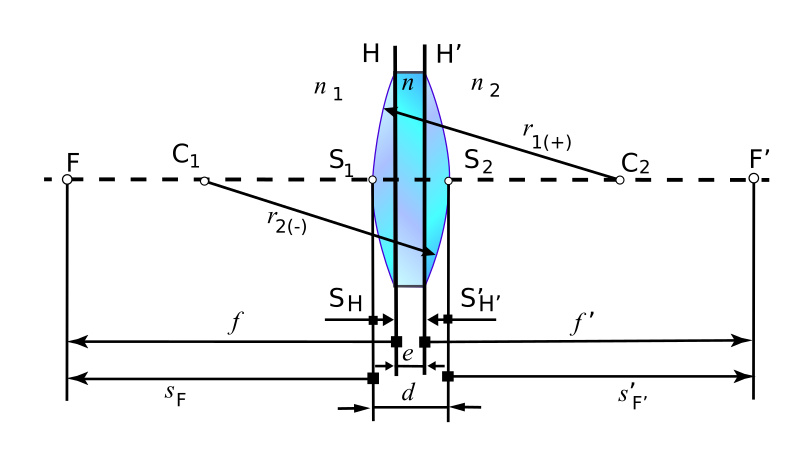
\includegraphics[width=1\linewidth]{Images/Week 1/Thick_Lens_Diagram.svg.png}
    \caption{Thick lens diagram}
    \label{fig:lens-diagram}
\end{figure}
For a thick lens, or systems consisting of several lenses, there are several related concepts that are referred to as focal lengths:
\begin{itemize}
    \item \textbf{Effective focal length (EFL)}: The EFL is the inverse of the optical power of an optical system, and is the value used to calculate the magnification of the system. The imaging properties of the optical system can be modelled by replacing the system with an ideal, thin lens with the same EFL. It also provides a simple method for finding the nodal points without tracing rays.
    \item \textbf{Fron focal length (FFL)}: The FFL $f$ is the distance from the front focal point $F$ to the front principal plane $H$
    \item \textbf{Rear focal length (RFL)}: The RFL, $f'$, is the distance from the rear principal plane $H'$ to the rear focal point $F'$.
    \item \textbf{Front focal distance (FFD)}: The FFD, $s_F$, is the distance from the front focal point of the system, $F$, to the vertext of the first optical surface $S_1$. Sometimes this is referred to as the front focal length.
    \item \textbf{Back focal distance (BFD)}: BFD, $s'_F$, is the distance from the vertex of the last optical surface of the system $S_2$ to the rear focal point $F'$. This is sometimes referred to as the back focal length.
\end{itemize}
For an optical system in the air, the above are all the same and may be called the focal length.
\newline \newline
For optical systems in mediums other than air or vacums, the focal length changes with the refractive index of the mediums, however, this project will not focus on this specific topic.

Camera lens focal lengths are usually specified in millimetres (mm), but some older lenses are marked with centimetres (cm) or inches.
\textbf{Focal length} $f$ and \textbf{field of view} of a lens are inversely proportional. For a standard recilinear lens,
\begin{equation}
    FOV = 2\arctan(\frac{x}{2f})
    \label{eq:fov}
\end{equation}
where $x$ is the width of the film or imaging sensor. When a photographic lens is set to "infinity", its rear principal plane is separated from the sensor or film, which is then situated at the focal plane, by the lens' focal length. Objects far away from the camera then produce sharp images on the sensor or film, which is also at the image plane.
\newline \newline
To render closer objects in sharp focus, the lens must be adjusted to increase the distance between the rear principal plane and the film, to put the film at the image plane. The focal length $f$, the distance from the front principal plane to the object to photograph $s_1$, and the distance from the rear principal plane to the image plane $s_2$ are then related by \(1/s_1 + 1/s_2 = 1/f\).
As $s_1$ is decreased, $s_2$ must be increased. For example, consider a normal lens for a 35mm camera with a focal length of $f=50$mm. To focus a distant object ($s_1 \approx \infty$), the rear principal plane of the lens must be located at a distance $s_2=50$mm from the film plane, so that it is at the location of the image plane. To focus an object 1m away ($s_1 = 1,000$mm), the lens must be moved 2.6mm farther away from the film plane, to $s_2=52.6$mm.

\subsection{Optical power}

The \textbf{optical power} of a lens or curved mirror is a physical quantity equal to the reciprocal of the focal length, expressed in metres. A dioptre is its unit of measurement iwth dimension of reciprocal length, equivalent to one reciprocal metre, 1 dioptre = 1$m^{-1}$. E.g., a 2-dioptre lens brings parallel rays of light to focus at $1/2$ metre. A flat window has an optical power of zero dioptres, as it does not cause light to converge or diverge.

\subsection{Field of view}
The \textbf{field of view (FOV)} is the angular extent of the observable world that is seen at any given moment. In photography, the FOV is that part of the world that is visible by the camera at a particular position and orientation in spacel objects outside the FOV when the picture is taken are not recorded in the photograph. It is most often expressed as the angular size of the view cone, as an angle of view. For a normal lens focused at infinity, the diagonal FOV can be calculated with \ref{eq:fov}.
\newline \newline
FOV is critically important in space imaging because it directly impacts what, how much, and how well a spacecraft or satellite can observe. Wider FOVs capture larger areas, whereas narrower FOVs capture more detail over a smaller area. For CubeSat applications, the FOV directly impacts the design on the system because a narrower FOV requires a longer focal length and a longer lens. If the FOV is too narrow, then deployable instruments must be investigated to break the 10x10x10cm constraint.
Wider FOVs don't require many manouvres to capture images, but narrow FOVs require precise movements to capture the correct area. Both have benefits and drawbacks.

\subsection{Aperture}
In optics, the aperture of an optical system is the hole or opening that primarily limits light propagated through the system. An optical system typically has many structures that limit pencils of light. These structures may be the edge of a lens, or a ring or other fixture that holds an optical element in place or may be a special element such as a diaphragm placed in the optical path to limit the light admitted by the system.
In general, these structures are called stops, and the aperture stop is the stop that primarily determines the cone of rays that an optical system accepts. As a result, it also determines the ray cone angle and brightness at the image point. The aperture stop generally depends on the object point location; on-axis object points at different lateral locations at the same object plane have different aperture stops (vignetted). In practice, many object systems are designed to have single aperture stop at designed working distance and field of view.
\newline \newline
The size of the aperture stop determines the amount of light admitted by an optical system. The aperture stop also affects other optical system properties:
\begin{itemize}
    \item The opening size of the stop is one factor that affects the \textbf{depth of field (DOF)}. A smaller stop (larger f number) produces a longer DOF because it only allows a smaller angle of the cone of light reaching the image plane so the spread of the image of an object point is reduced. A longer DOF allows objects at a wide range of distances from the viewer to be in focus at the same time.
    \item The stop limits the effect of optical aberrations by limiting light such that the light does not reach edges of optics where aberrations are usually stronger than the optics centers.
    \item The stop determines whether the image will be vignetted. Larger stops can cause the light intensity reaching the film or detector to fall off toward the edges of the picture, especially when, for off-axis points, a different stop becomes the aperture stop by virtue of cutting off more light than did the stop that was the aperture stop on the optic axis.
    \item The stop location determines the telecentricity (the entrance or exit pupil, or both, at infinity). If the aperture stop of a lens is located at the front focal plane of the lens, then it becomes image-space telecentricity, i.e., the lateral size of the image is insensitive to the image plane location. If the stop is at the back focal plane of the lens, then it becomes object-space telecentricity where the image size is insensitive to the object plane location. The telecentricity helps precise two-dimensional measurements because measurement systems with the telecentricity are insensitive to axial position errors of samples or the sensor.
\end{itemize}
In astronomy, the opening diameter of the aperture stop (called the aperture) is a critical parameter in the design of a telescope. Generally, you would want the aperture to be as large as possible, to collect the maximum amount of light from the distant objects being imaged. The size of the aperture is limited, however, in practice by considerations of its manufacturing cost and time and its weight, as well as prevention of aberrations (as mentioned above).
\newline \newline
In photography, the aperture stop of a photographic lens can be adjusted to control the amount of light reaching the image sensor. In combination with variation of shutter speed, the aperture size will regulate the image sensor's degree of exposure to light (this is called the \href{https://photographylife.com/what-is-exposure-triangle}{exposure triangle}). A device called a diaphragm usually serves as the aperture stop and controls the aperture. The diaphragm serves much like the iris of the eye. Reducing the aperture size provides less light to the sensor and increases the depth of field, which describes the extent to which subject matter lying closer than or farther from the actual plane of focus appears to be in focus.
The lens aperture is usually specified as an f-number, the ratio of focal length to effective aperture diameter. In photography, \textit{one f-stop} refers to a factor of $\sqrt{2}$ change in f-number which corresponds to a $\sqrt{2}$ change in aperture diameter, which in turn corresponds to a factor of 2 change in light intensity (by a factor 2 change in the aperture area).
The amount of light captured by an optical system is proportional to the aera of the entrance pupil that is the object space-side image of the aperture of the system, equal to:
\[
Area = \pi (\frac{D}{2})^2 = \pi (\frac{f}{2N})^2
\]
Where the two equivalents are related by the f-number $N=f/D$, with focal length $f$ and entrance pupil diameter $D$.

\subsection{Key Trade-Offs in Earth Observation Imaging}
The interplay between motion blur, exposure time, and depth of field is a critical consideration in Earth observation imaging. Adjusting one parameter often impacts the others, necessitating a balance to achieve optimal image quality.
\newline \newline
\textbf{Motion Blur vs. Exposure Time}: Longer exposure times capture more light, reducing noise, but they increase the risk of motion blur, especially in satellite imaging where relative motion is significant. Conversely, shorter exposure times minimise motion blur but may lead to darker images since they capture less light. The maximum exposure time to minimise motion blur can be found by \(t=\frac{rc}{v}\), where $r$ is the spatial resolution, $c$ is a factor of the motion blur (between 0 and 1) and $v$ is the speed of the CubeSat.
\newline \newline
\textbf{Exposure Time vs. Noise}: Reducing exposure time to combat motion blue can result in increased image noise, as the sensor has less time to collect photons. This trade-off is particularly challenging in low-light conditions or when high image clarity is required.
\newline \newline
\textbf{Aperture vs. Exposure}: A wider aperture allows more light, enabling shorter exposure times and reducing motion blur. However, it decreases the depth of field, potentially causing parts of the image to be out of focus. A narrower aperture increases depth of field but required longer exposure times.
\newline \newline
Advanced sensors with higher sensitivity (quantum efficiency) can mitigate some of these trade-offs by allowing shorter exposure times without significantly increasing noise. Techniques such as motion compensation and image stabilisation can help reduce the effects of motion blur without altering exposure settings. Image processing algorithms can correct for certain artifacts like noise and blur, but they have limitations and cannot fully compensate for suboptimal capture settings.

\subsection{C, CS and S-Mount Camera Lenses}
Lens mounts are the mechanical interfaces that attach a lens to a camera and set the correct distance for focus. When designing compact or modular camera systems, three primary lens mount types are commonly considered: \textbf{M12 (S-Mount), CS-mount}, and \textbf{C-mount}. Each has distinct mechanical and optical characteristics, making them suitable for different use cases.
\newline \newline
The \textbf{M12 mount}, also known as the \textbf{S-mount}, is the smallest and lightest of the three. It uses a 12mm diameter thread and has no fixed flange focal distance (FFD), typically relying on adjustable back-focus. M12 lenses are compact and inexpensive, making them ideal for small embedded systems like drones or hobby cameras. However, their image quality is generally lower due to smaller optics, and they usually support sensor formats up to 1/2" or 1/1.8".
\newline \newline
The \textbf{CS-mount} is a more robust, standardised system commonly used in CCTV and industrial vision. It shares the same thread as the C-mount (1"-32 UN), but has a shorter FFD of 12.5mm, which means lenses sit closer to the sensor. CS-mount cameras can use both CS and C-mount lenses, giving it some flexibility. These lenses support larger sensors and generally offer better image quality than M12 lenses.
\newline \newline
The \textbf{C-mount} is the most optically capable of the three, also using the 1"-32 UN thread0 but with a 17.526mm FFD. C-mount lenses are larger, heavier, and typically of higher optical quality, supporting sensor sizes up to 1" or more. They are often used in scientific imaging, space optics, and high-end industrial systems. However, their size and mass can be a limiting factor in space-constrained environments.

\subsection{Autofocus vs. Fixed-focus Lenses}
Embedded vision systems rely heavily on the capabilities of their lenses. The lens's optical properties, such as its focal length, aperture, and FOV, dictate the clarity, depth, and breadth of the captured image. These parameters, along with sensor size and resolution, directly impact the systems' ability to analyse and interpret visual data.
\newline \newline
A \textbf{fixed-focus lens} comes with a determined and unchangeable focal length. Once set, this focus remains constant and doesn't adjust based on changes in the scene or the distance of the target object. Such lenses are calibrated during the design or manufacturing phase for a specific application or distance, ensuring optimal clarity for that designated range.
Fixed-focus lenses are advantageous in scenarious that demand consistent and predictable imaging results. When objects are presented at a consistent distance from the camera, fixed-focus lenses offer stability and repeatability. For the CubeSat mission, it is highly likely we will used a fixed-focus lens since we will only be taking one type of image at a consistent orbital distance.
\newline \newline
An \textbf{autofocus (AF)} lens can automatically adjust its focus based on the scene. Unlike manual focus lenses, which require a predefined focus set during the design or intial setup, autofocus lenses dynamically adjust to ensure the targeted subject or region of interest remains sharp. It is achieved through sensors and algorithms that detect the optimal focus point, allowing the lens to modify its focus in real time.
AF lenses offer a high level of adaptability and accuracy in embedded vision systems, ranging from industrial automation to medical devices. They can continuously adjust to provide sharp images.
\newline \newline
The selection criteria for AF vs. fixed-focus lens includes:
\begin{itemize}
    \item \textbf{Proximity}: The distance between the camera and target plays a crucial role in selecting a lens, impacting the clarit and precision of captured images. AF lenses are preferable for fluctuating distances, especially from a close 10cm to an endless range, allowing dynamic adjustments. However, a fixed-focus lens is better suited for a set distance, ensuring consistent imagery without any adjustments.
    \item \textbf{Depth of Field (DoF)}: Cameras with autofocus lenses offer broader field depths than their fixed-focus counterparts. But sometimes, depending on the use case, a fixed-focus camera lens may be required, as some applications do not need broader field depths.
    \item \textbf{Lighting Conditions}: This directly influences the clarity of photos. Autofocus lenses perform better under low lighting, with some fine-tuning to provide further clarity. However, under brightly lit conditions, a fixed-focus camera lens can offer clear images within its preset range.
    \item \textbf{Rate of capture}: Fixed-focus lenses typically work faster than their AF counterparts, as they lack the need for focus adjustments. Their design prioritises speed over adaptability, making them efficient for certain tasks. Consequently, if an application demands fast image cpature without interruptions, a fixed-focus lens is the recommended choice. It ensures consistent, rapid imaging without the potential lag of autofocus lens adjustments.
    \item \textbf{Adaptability}: The camera lens' versatility is also a deciding factor. Autofocus lenses perform better in low-light scenarios, with some customisation. However, fixed-focus camera lenses can offer clear images within their preset range under brightly lit conditions, where light is stable and abundant.
\end{itemize}
With the CubeSat mission in mind, these considerations are critically important:
\begin{itemize}
    \item \textbf{Size and Weight}: AF lenses require motors, actuators, and additional housing, all of which increase the overall size and mass. Fixed-focus lenses are typically much smaller and lighter.
    \item \textbf{Power Consumption}: AF systems consume electrical power to operate motors and sensors needed for focusing. Fixed lenses use no power once installed.
    \item \textbf{Reliability}: Moving parts in AF lenses can jam, degrade, or fail over time. A foxed-focus system is mechanically simple and has fewer points of failure, making it much more suitable for long-duration, unattended missions.
    \item \textbf{Launch Survivability} The vibration during rocket launch can damage sensitive optical systems. AF components may loosen or break. Fixed-focus lenses are more robust and more likely to survive launch intact.
    \item \textbf{Autonomy and Complexity}: AF systems require logic to detect blur, estimate distance, and control motors. This demands more computing resources and software development. Fixed-focus lenses avoid this entirely, simplifying the onboard system and reducing potential bugs.
\end{itemize}
As previously mentioned, it is very likely the CubeSat mission will utilise a fixed-focus lens. Future missions may provide scope to consider AF systems, however, since the projected outcomes for the first CubeSat mission involve functionality of the core sub-systems, a fixed-focus lens will be best suited to the mission.

\subsection{Wide and vs. Telephoto Imaging}
\textbf{Telephoto imaging} refers to a narrow FOV with high magnification (useful for capturing small details or distant targets), whereas \textbf{wide-angle imaging} provides a broader FOV (useful for capturing a larger area).
\newline \newline
Telephoto lenses require a much larger focal length which is difficult to achieve in a CubeSat form factor. There have recently been \href{https://digitalcommons.usu.edu/cgi/viewcontent.cgi?referer=&httpsredir=1&article=3059&context=smallsat}{developments} into deployable telephoto lenses to achieve extremely high levels of detail up to 1 metre per pixel. These missions can typically use a 2U or larger form factor, so reaching a relatively high level of spatial resolution (50-100 metres per pixel) is a strong possibility for the CubeSat mission. Deployable telescopes may be out of scope for this first CubeSat mission, however, they do demonstrate that the task is possible.
Since longer focal lengths require a higher frame stability, more power may need to be directed to the ADCS. Telephoto imaging means the camera must be pointed very precisely at the target. Error in attitude can cause motion blur, data loss or missing the target entirely. Achieving this requires a longer stabilisation time after manouvres to confirm attitude.
Custom telephoto lens systems require more planning, budget, stricter testing and longer development times because of the increased scope.
\newline \newline
\textbf{Wide angle lenses} have a much shorter focal length and their optical systems are much more compact. The wider FOV loses detail since the spatial resolution is much larger, however, they capture a larger area.
These lenses tolerate pointing errors because of the low spatial resolution. If the CubeSat isn't facing the target by a couple degrees, or is slowly rotating, the image will most likely be unaffected because the wide FOV tolerates more errors e.g., accidentally pointing at Mandurah instead of Perth doesn't matter if we are capturing an image from Esperance to Shark Bay.
Additionally, COTS wide angle cameras are cheap, small and readily available which will make integration much easier.
\newline \newline
Since the file size and thermal management of both camera systems would be similar, it is not a critical comparison consideration.

\subsection{Optical distortions and corrections}
Distortion is specified as a percentage of the field height. Typically, $\pm 2\%$ to $3\%$ distortion is unnoticed in a vision system if measurement algorithms are not used. In simple lenses, there are two main types of distortion: negative, barrel distortion, where points in the FOV appear too close to the center; and positive, pincushion distortion, where points are too far away. Barrel and pincushion refer to the shape of the field when distorted, shown in \ref{fig:lens-distortion}.
\begin{figure}[H]
    \centering
    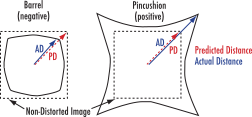
\includegraphics[width=0.6\linewidth]{Images/Week 1/distortion-2.png}
    \caption{An illustration of positive and negative distortion.}
    \label{fig:lens-distortion}
\end{figure}
These are usually referred to as \textbf{geometric distortions}, because straight lines appear curved or displaced especially at wide angles or at the edges of the FOV.
Distortion is calculated simply by relating the actual distance (AD) to the predicted distance (PD) of the image using \ref{eq:distortion}.
\begin{equation}
D(\%)=\frac{AD-PD}{PD}\times100\%
    \label{eq:distortion}
\end{equation}
These usually occur when the magnification decreases with distance from the center and is common in wide-angle and cheap lenses. Fortunately, some software algorithms like OpenCV's undistort() can provide optical correction (some applications such as Photoshop and Matlab have lens profiles in the software).
\newline \newline
\subsubsection{Fisheye Distortion}
\textbf{Fisheye Distortion} is an extreme wide-angle effect where lines are heavily cirved, giving a hemispherical apperance. This is usually intentional for fish-eye lenses to capture extremely wide FOVs of $>160$\textdegree. Sometimes the effect is desirable, but it can be correct via software remapping using known distortion models (e.g., Photoshop has options to reverse fish-eye lens effects).
\newline \newline
Optical aberrations are performance deviations from a perfect, mathematical model. It is important to note that they are not cause by manufacturing flays, physical, optical, nor mechanical. Rather, they are inherent in lens design and are due to diffraction, refraction, and the wave nature of light. As such, there is no perfect lens.
Effects from various aberrations in a lens design are ultimately seen in performance and affect modulation transfer function (MTF), spot size, telecentricity, DOF, and others. Aberration theory is an abstract and complex subject. Understanding how aberrations affect performance is important for success with an application.
Whilst aberration theory is a vast subject, basic knowledge of a few fundamental concepts can ease understanding: spherical, astigmatic, field curvature and chromatic.
\newline \newline
\subsubsection{Spherical Aberration}
\textbf{Spherical Aberration} refers to rays focusing at different distances depending on where they interact with the lens and is a function of aperature size. To describe spherical aberration, the incident angle of light must be known. This angle occurs where light rays strike the curved surface of a lens and is the angle between the ray and the surface. The steeper the incident angle, the more light will be refracted.
\begin{figure}[H]
    \centering
    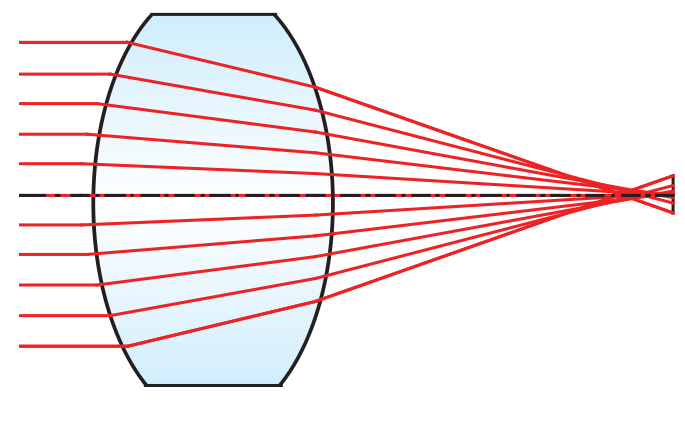
\includegraphics[width=0.8\linewidth]{Images/Week 1/spherical-abberation.png}
    \caption{An example of spherical aberration. The light incident upon the edges of the lens focuses more quickly due to their higher angle of incidence. Note that rays closer to the optical axis (smaller angle of incidence refract less).}
    \label{fig:spherical-aberration}
\end{figure}
\ref{fig:spherical-aberration} shows that as the parallel rays in object space collide with the lens, the incident angle increases the farther up they hit on the lens's surface. Image quality from the lenses with large apertures are more likely to suffer from spherical aberration, because of this larger angle of incidence. Lenses that suffer from spherical aberration can be improved by increasing the f-stop by closing the iris. Closing the iris too much causes diffraction to limi performance sooner. Optical designs that include high index glass or additional elements are used to correct spherical aberration in a fast (small f-stop) lens; these designs reduce the amount of refraction at each surface and, with it, the amount of spherical aberration. However, this increases the size, weight, and cost of the lens assembly.
\newline \newline
\subsubsection{Astigmatism}
\textbf{Astigmatism} is a function of field angles. To summarise, astigmatic aberration occurs when a lens must perform over a wide field, but the performance in the direction of the field is reduced compared to the performance orthogonal to the field (either sagittal or tangential, respectfully). If one looks at a series of bars that are half horizontal (tangential) and half vertical (sagittal), the bars in one direction will be in focus, but the bars in the other will be out of focus.
\begin{figure}[H]
    \centering
    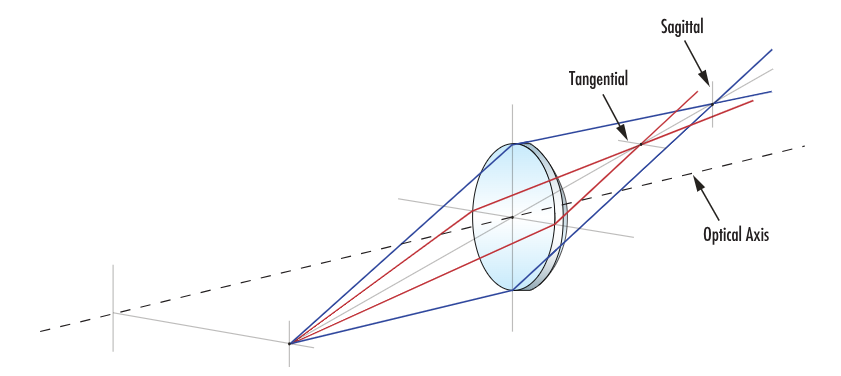
\includegraphics[width=0.8\linewidth]{Images/Week 1/astigmatism.png}
    \caption{Off-axis asymmetry. Note that the tangential and sagittal points of focus are different.}
    \label{fig:astigmatism}
\end{figure}
This is caused by the fact that the rays that are away from the center of the object, do not pass through rotationally symmetric surfaces like the on-axis rays do in \ref{fig:astigmatism}. To correct this, two things must occur: lens designs must be symmetric about the aperture and field rays must have low incident angles. Keeping a design symmetric leads to forms that are like a double gauss lens. Note that symmetric designs prevent the use of telephoto or reverse telephoto designs, which can cause long focal length designs to be large and short focal length designs to have small back focal lengths. Reducing the angles of incidence, much like for spherical aberration, requires higher index glasses and additional elements, leading to an increase in lens size, weight, and cost. The simplified definition used here intentionally combines the effects of astigmatism and coma for ease of understanding.
\newline \newline
\subsubsection{Field Curvature}
\textbf{Field Curvature} is the aberration that describes the amount in which the image plane curves due to the curvature in the lens design. This aberration is caused by the sum of the focal lengths of the lens elements in the system (multiplied by the refractive indices) not equalling zero. If the sum is positive (typical for an imaging lens), the image plane will have a concave curvature. Since curving the image plane is almost never an option for a machine vision lens, the optical designer must insert negative powered corrective elements to reduce this sum. This makes lenses longer and forces a negative lens to be close to the image plane, reducing the lens's back focal length.
\begin{figure}[H]
    \centering
    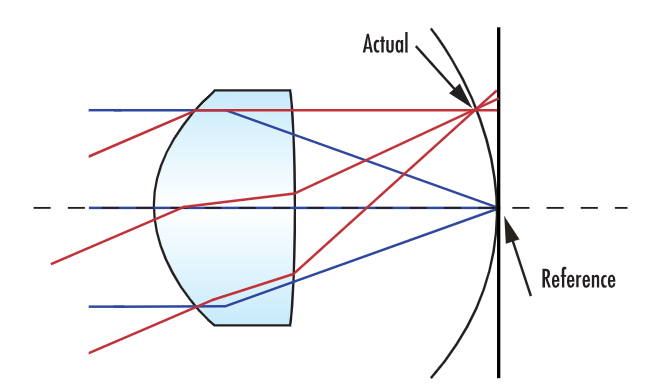
\includegraphics[width=0.8\linewidth]{Images/Week 1/curvature.png}
    \caption{A field curvature example showing the non-planer surface of best focus.}
    \label{fig:curvature}
\end{figure}
\subsubsection{Chromatic aberration}
\textbf{Chromatic aberration} occurs when light of different wavelengths focus at different points since the refractive index of glass varies based on the wavelength of light. Lenses using longer wavelengths of light have relatively longer focal lengths than lenses using shorter wavelengths. Because the dispersion of a glass determines the refractive power of the glass at different wavelengths, chromatic aberration can be removed by designing an imaging lens that contains both positive and negative lenses made using glasses with different dispersions. This is shown in \ref{fig:chromatic}, which compares a singlet to an achromatic doublet lens.
\begin{figure}[H]
    \centering
    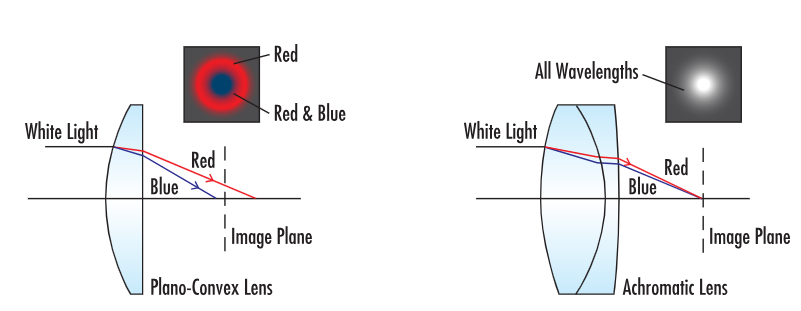
\includegraphics[width=0.8\linewidth]{Images/Week 1/chromatic.png}
    \caption{A comparison of singlet and doublet lens spots.}
    \label{fig:chromatic}
\end{figure}
A downside to such a design is the increase in the number of lens elements used. To reduce the aberration, lower index lenses are needed to correct spherical and astigmatic, and chromatic aberrations; if corrections for spherical, astigmatic, and chromatic aberrations must be done, additional lens elements are needed. Additionally, the most desirable glasses for color correction often have properties that make them more expensive and difficult to manufacture. Minimising chromatic aberration by using monochromatic light has considerable savings in cost and complexity.
\newline \newline
\subsubsection{Chromatic Focal Shift}
\textbf{Chromatic Focal Shift} is a type of chromatic aberration, chromatic focal shift describes how different wavelengths focus along different longitudinal positions (along the optical axis). The goal of most imaging lens designs is to have all desired wavelengths focus on the same plane (where the sensor is located). It is physically impossible to get a singular focus plane over a wide spectral range. However, it is possible to come close. If the wavelengths are focused closer to the same plane, fewer issues will be observed in the image.
\begin{figure}[H]
    \centering
    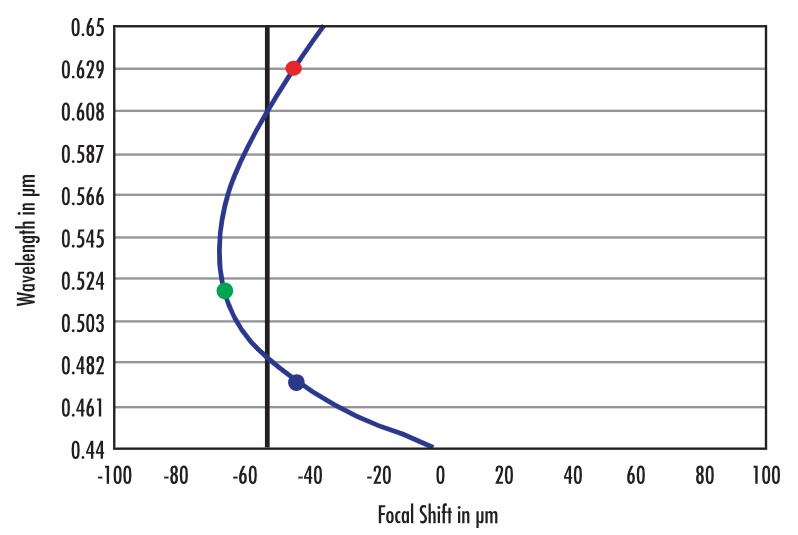
\includegraphics[width=0.8\linewidth]{Images/Week 1/achromat.png}
    \caption{Chromatic focal shift curve for an achromatic lens.}
    \label{fig:achromat}
\end{figure}
\ref{fig:achromat} shows a chromatic focal shift curve. Since this is an example of an achromatic lens design, two wavelengths are focused on the same plane. The y-axis shows changing wavelength from short to long (blue to red in the visible spectrum). The vertical black line represents a plane that could be the sensor location, and the x-axis shows the distance away from that location. The blue curved line shows the relative location of the best focus as a function of wavelength. The curve verifies that this design is achromatic since even if moved slightly to the left or right, the black line intersects the blue curve at only two points/wavelengths.
The blue, green, and red dots represent wavelengths associated with common 470nm, 520nm, and 630nm (blue, green, and red) LEDs. Notice the green dot focuses to the left of the sensor plane, while the red and blue dots focus to the right; this is the most balanced position of focus of the lens system if all the wavelengths or white light (which encompasses all wavelengths) are used. This design displays non-ideal image quality, as none of the wavelengths are truly in focus. If only one wavelength is used, the performance will improve since balancing effects used for the other wavelengths are eliminated. While this example demonstrates that red and blue can be balanced, this is not always true. Most lens designs are achromatic, but for very small pixels, this can be an issue.
\begin{figure}[H]
    \centering
    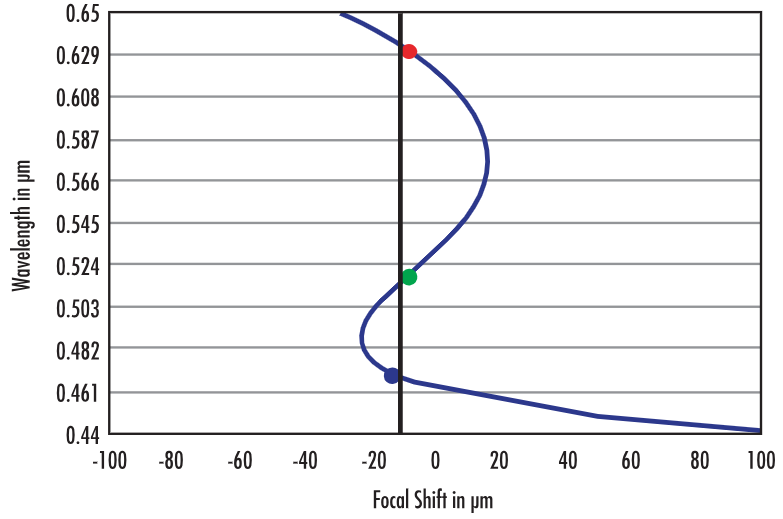
\includegraphics[width=0.8\linewidth]{Images/Week 1/apochromat.png}
    \caption{Chromatic focal shift for an apochromatic lens.}
    \label{fig:apochromat}
\end{figure}
Shown at the same scale as \ref{fig:achromat}, \ref{fig:apochromat} shows an apochromatic lens. An apochromatic lens is designed to focus three wavelengths on the same plane. While this is a far more complicated design, it allows for superior balancing across the wavelength spectrum. As shown, all three LED colors can be brought to focus on the same sensor plane allowing for superior image quality. Apochromatic lens designs have high performance, but low versatility and work well over a smaller range of magnifications and WDs. Additionally, these are often high-cost designs due to additional elements made of expensive materials. Many high-end, high-magnification objectives (such as microscope objectives) are apochromatic.

\subsection{Filter types}
\subsubsection{IR-cut filters}
Generally, systems such as CMOS and CCD cameras capture accurate images in daylight. Their sensors can detect near-infrared light that is invisible to the human eye. Whilst this can be an important feature for night-vision recording, the infrared light distorts the colours of recorded images during daytime hours.
\newline
\textbf{Infrared (IR) cut filters} are a mechanical shutter design that blocks or delivers the IR, providing a high quality image with true colour reproduction, irrespective of day or night. To make images more similar to waht humans can view, most OEM cameras are fitted with an IR-cut filter which allows only the visible light to pass through, thereby reflecting the unwanted IR.
\begin{figure}[H]
    \centering
    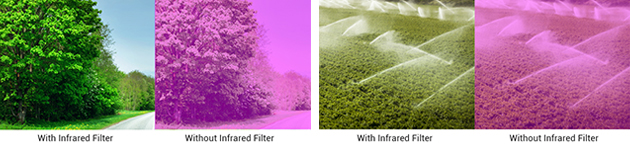
\includegraphics[width=0.8\linewidth]{Images/Week 1/IR-cut.jpg}
    \caption{Comparison of images with and without IR-cut filter.}
    \label{fig:IR-cut}
\end{figure}
\begin{figure}[H]
    \centering
    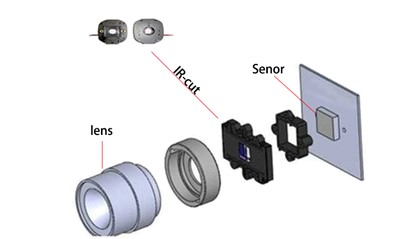
\includegraphics[width=0.8\linewidth]{Images/Week 1/IR-cut-diagram.jpg}
    \caption{Placement of IR-cut filter in a camera}
    \label{fig:IR-cut-diagram}
\end{figure}
The filter is controlled by a motor or with the help of an electromagnet. When the IR filter is turned on during daytime, it helps to block IR, letting only the visible light pass through. This process is known as \textbf{True Day Night (TDN)} because it delivers true colour images during the day and black and white or night vision images at night. It ensures that the image colours are not disturbed and generates a true representation of colours, as seen by naturally by the human eye.
When the IR filter is turned off during the night or in low-light confitions, it helps IR and other forms of light to reach the CCD/CMOS sensor. The image sensor, in turn, absorbs enough light, and the camera turns back to black-and-white mode, which is more sensitive to IR light.
\newline \newline
There are three main reasons to use an IR-cut filter:
\begin{itemize}
    \item \textbf{To avoid colour distortion}. Generally, IR light leads to colour distortion during the day. To solve this issue, an IR-cut filter is used to keep the IR light disturbance out of the image sensor during the day. When the light falls below a certain level, the filter automatically swivels out of the way so that the IR light does hit the image sensor. Also, the camera switches to black-and-white mode to use the IR light optically.
    \item \textbf{To achieve realistic colours}. The IR-cut filter in a colour camera can achieve realistic colours in white light. In general, the colour spectrum viewed by the human eye is quite limited compared to the sepctrum viewed by a CCD camera. Especially, the difference in sensitivity is significant in the near IR region of the spectrum. If an IR-cut filter is not used, a huge amount of infrared light will appear, resultin in strange colours.
    \item \textbf{To achieve colour correction in lenses}. In many cases, it is difficult to design imaging optics covering both the visible sepctrum and the near IR spectrum. Therefore, many lenses have different depths of focus for the visible and the IR spectrum. In such cases, the IR-cut filter cuts away a significant amount of the collected light and achieves colour correction in lenses.
\end{itemize}
\begin{figure}[H]
    \centering
    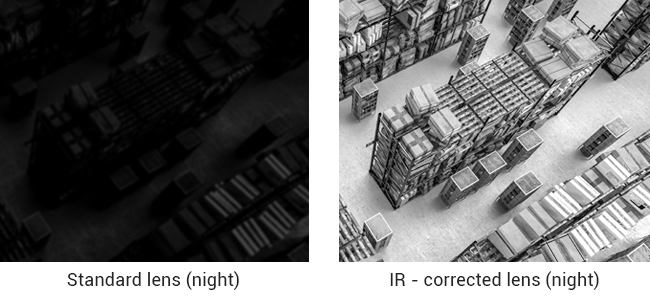
\includegraphics[width=0.8\linewidth]{Images/Week 1/IR-day-night.jpg}
    \caption{Comparison of standard lens and IR-corrected lens}
    \label{fig:IR-day-night}
\end{figure}
\subsubsection{Bayer filters vs. monochrome sensors}
\textbf{Bayer filters} and \textbf{monochrome sensors} are distinct approaches to image capture in digital cameras. Bayer filters are used in standard colour cameras to capture colour information, while monochrome sensors capture only light intensity without colour information. This leads to differences in image quality, low-light performance, and resolution.
\newline \newline
Bayer filters, also known as \textbf{Colour Filter Arrays (CFAs)} are used to create colour images. They consist of a mosaic of red, green and blue filters arranged over the sensor's pixels.
Each pixel in a Bayer sensor captures only one colour component. To create a full-colour image, the missing colour information for each pixel is interpolated from its neighbours, a process that can introduce some softness or artifacts.
Bayer filters are the standard for most digital cameras and camcorders.
\begin{figure}[H]
    \centering
    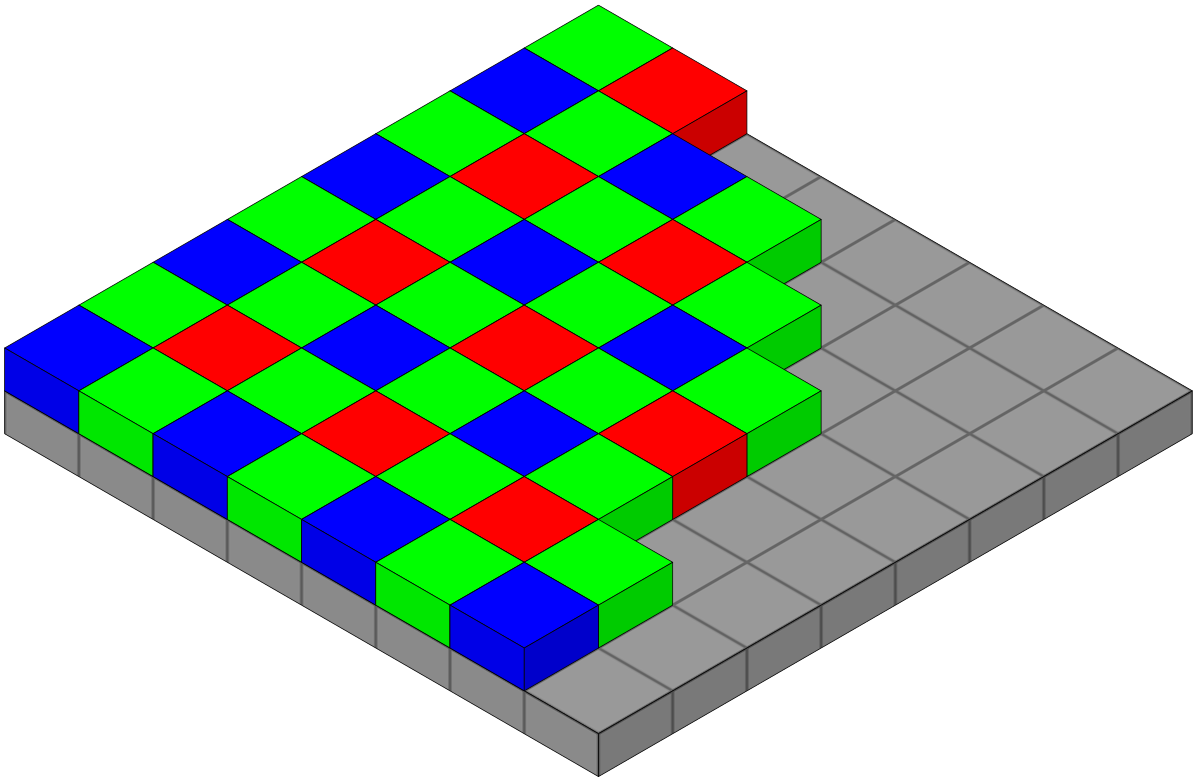
\includegraphics[width=0.8\linewidth]{Images/Week 1/bayer-pattern.png}
    \caption{Simple Bayer sequence of RGGB.}
    \label{fig:bayer-sequence}
\end{figure}
As shown in \ref{fig:bayer-sequence}, bayer filters use a RGGB sequence to emulate the vision of the human eye since we are more sensitive to green light compared to red and green.
Unfortunately, the colour filter array reduces the amount of light reaching the sensor, potentially impacting low-light performance. Interpolation can also slightly reduce sharpness compared to monochrome sensors.
Fortunately, they provide the ability to capture full colour information in a single shot.
\newline \newline
Monochrome sensors only capture the intensity of light without any colour filtering. Because they capture all the light information at each pixel, monochrome sensors can provide higher resolution and finer detail compared to Bayer sensors, especially in low-light conditions.
Without the light-absorbing colour filters, monochrome sensors are more sensitive to light, making them better in low-light situations. They are favoured in scientific, industrial and specialised applicants where colour information is not essential.
Although they capture only greyscale images, monochrome sensors can also be used with filters to create different black and white looks. They also offer greater flexibility in post-processing for contrast and tone adjustments.
Since there is no need for colour interpolation, monochrome sensors can offer sharper images with more detail.

\subsubsection{Bandpass \& ND filters}
\textbf{Bandpass} and \textbf{Neatural Density (ND)} filters are crucial in imaging missions for enhancing image quality, controlling light, and enabling specific observations. Bandpass filters isolate specific wavelengths of light, improving contrast and clarity, while ND filters reduce overall light intensity, preventing sensor saturation in bright conditions and allowing for longer exposure times.
\newline \newline
Bandpass filters selectively transmit a specific range of wavelengths while blocking others, which is useful for isolating specific features or phenomena in an image. Some of the applications include:
\begin{itemize}
    \item \textbf{Astronomy}. Enhancing contrast in images of nebulae and galaxies by isolating specific emission lines.
    \item \textbf{Fluroescence microscopy}. Isolating excitation and emission wavelengths to visualise specific biological molecules.
    \item \textbf{Machine vision}. Improving contrast and resolution by reducing chromatic aberration and selecting relevant wavelengths.
    \item \textbf{Environmental monitoring}. Detecting specific gases or pollutants based on their spectral signatures.
    \item \textbf{Remote sensing}. Identifying materials and vegetation based on their unique spectral reflectance.
\end{itemize}
Some of the benefits include:
\begin{itemize}
    \item \textbf{Improved Signal-to-Noise (SNR) ratio}. By blocking unwanted light, bandpass filters enhance visibility of the desired signal.
    \item \textbf{Enhanced contrast and clarity}. Isolating specific wavelengths allows for clearer visualisation of target features.
    \item \textbf{Precise spectral analysis}. Bandpass filters are essential for spectroscopic analysis and identifying chemical compositions.
\end{itemize}

ND filters reduce the intensity of all wavelengths of light equally, allowing for slower shutter speeds or wider apertures in bright conditions. Some of the applications include:
\begin{itemize}
    \item \textbf{Daytime photography and videography}. Preventing overexposure in bright sunlight and enabling creative effects like motion blur.
    \item \textbf{Long-exposure photography}. Allowing for long exposures in daylight to capture light trails or smooth water.
    \item \textbf{Drone imaging}. Controlling exposure in aerial photography and videography.
\end{itemize}
Some of the benefits include:
\begin{itemize}
    \item \textbf{Controlled exposure}. ND filters allow for proper exposure in bright conditions, preventing sensor saturation.
    \item \textbf{Creative effects}. Enabling long exposures and motion blur in bright environments.
    \item \textbf{Sensor protection}. Reducing light intensity can help protect the sensor from damage in very bright conditions.
\end{itemize}

In some imaging missions, bandpass and ND filters are used together. For example, in drone imaging, a bandpass filter might be used to isolate secific spectral band for vegetation analysis, while an ND filter could be used to control the overall exposure level.
Dual bandpass filters can be used to optimise imaigng for both visible and near-IR light.

% -----------------------
% WEEK 2
% -----------------------

\section{Image Sensors \& Signal Conversion}
\subsection{Photodiodes}
Photodiodes are semiconductor devices that convert light into electrical current. When light, specifically photons, strike the photodiode's p-n junction, they generate electron-hole pairs. These carriers are then separated by the electric field in the depletion region, creating a photocurrent. The amount of current produced is directly related to the intensity of the incident light. 
\begin{figure}[H]
    \centering
    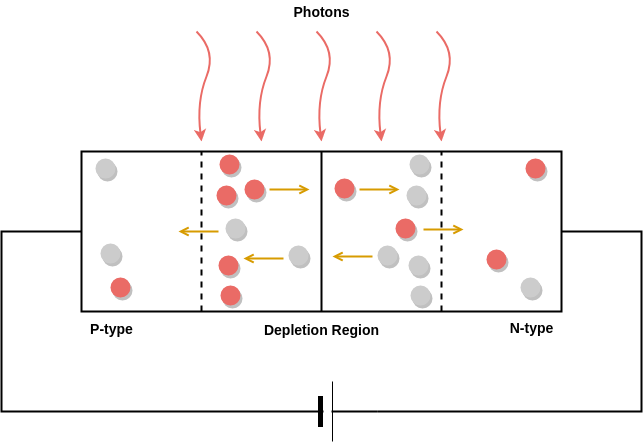
\includegraphics[width=0.8\linewidth]{Images/Week 2/photodiode.png}
    \caption{Photodiode diagram}
\end{figure}
Photodiodes can operate in two main modes:
\newline
\textbf{Photovoltaic mode}. In this mode, no external voltage is applied, and the photodiode generates a voltage when exposed to light.
\newline
\textbf{Photoconductive mode}. A reverse bias voltage is applied, increasing the depletion region and enhancing the photodiode's sensitivity and response speed.

\subsubsection{Photoelectric effect}
The photoelectric effect is the emission of electrons from a material caused by electromagnetic radiation such as ultraviolet light. Electrons emitted in this manner are called photoelectrons. The phenomenon is studied in condensed matter physics, solid state, and quantum chemistry to draw inferences about the properties of atoms, molecules and solids. The effect has found use in electronic devices specialised for light detection and precisely timed electron emission.
\newline \newline
The photoelectric effect is the core principle of how digital cameras operate. When a photon strikes the photodiode, it transfers energy to electrons in the material (typically silicon). This is a direct application of the photoelectric effect. These freed electrons are collected and stored as an electric charge in a potential well. The more photons hit the pixel, the more electrons accumulate, this is how brightness is measured. The camera's electronics read out the stored charges and convert them to digital values, which are processed to form the final image.

\subsubsection{Quantum efficiency}
\textbf{Quantum efficiency (QE)} in camera sensors refers to the percentage of incoming photons that are successfully converted into electrons, which are then used to form an image. A higher QE indicates a more efficient sensor, meaning it can produce a stronger signal from the same amount of light, leading to better image quality, particularly in low-light conditions. 
\newline \newline
QE is a crucial factor in determining a camera's sensitivity, especially in low-light situations. Higher QE leads to better signal-to-noise ratio, meaning a clearer, less noisy image, especially when light levels are low.
QE varies with the wavelength of light. Some sensors are more efficient at certain wavelengths than others. Different sensor technologies (e.g., CCD, CMOS, back-illuminated, front-illuminated) have varying QE characteristics. Back-illuminated sensors generally have higher QE than front-illuminated sensors, but they are also more expensive. 

\subsubsection{Charge accumulation}
In camera sensors, \textbf{charge accumulation} is the process where light is converted into electrical charge within tiny light-sensitive elements called pixels. This charge is accumulated proportionally to the intensity of the light striking each pixel during the exposure time. The accumulated charge is then read out and processed to create the final image. 
\newline \newline
In \textbf{Charge-Coupled Device (CCD)} sensors, the accumulated charge is transferred through the sensor's grid, like a bucket brigade, to a common readout circuit. 
In \textbf{Complementary Metal-Oxide-Semiconductor (CMOS)} sensors, the charge at each pixel is converted to a voltage, and then the signal is read out. 
The accumulated charge values from all pixels are then read out, converted into digital data, and processed by the camera's electronics to form the final image. 

\subsubsection{Full well}
A \textbf{full well} in an image sensor is the amount of charge that can be stored within an individual pixel without the pixel becoming saturated. It is dependent on the pixel size of the sensor and the camera operating voltages.
\begin{figure}[H]
    \centering
    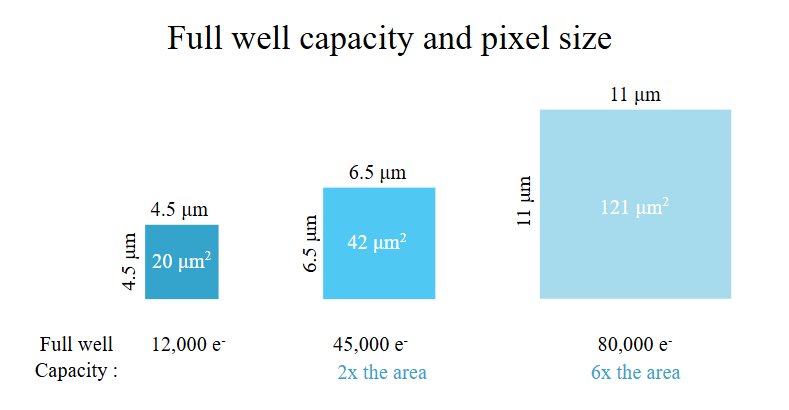
\includegraphics[width=1\linewidth]{Images/Week 2/full-well.png}
    \caption{Three different cameras with 2.5, 5 and 10 µm pixels. The full well capacity increases with increasing pixel size.}
\end{figure}
Different sized pixels are used for different applications. Whilst a smaller pixel size increases the number of pixels that can be placed on a sensor, the number of photons each pixel can detect is also reduced for the same photon flux, and therefore quantum efficiency tends to be reduced. Since fewer photons are collected the signal is lower and so the signal-to-noise ratio is reduced.
On the other hand, if the sensor is too big, or contains too many pixels, a much greater computational power is required to process the output information, decreasing image acquisition. It is important to select a camera sensor that balances the pixel size requirements with the acceptable noise levels for the application.
Generally, larger pixel sizes are used for achieving a higher sensitivity whilst smaller pixels are used for obtaining a higher spatial resolution.
\newline \newline
Below is a diagram of a general pixel - not specific to any sensor type. Please refer to this figure for concepts discussed later such as microlenses.
\begin{figure}[H]
    \centering
    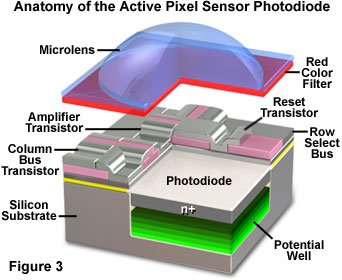
\includegraphics[width=1\linewidth]{Images/Week 2/pixel-diagram.png}
    \caption{See caption above.}
\end{figure}

\subsubsection{Saturation}
At the saturation point, pixels are unable to store additional charges, so instead this charge is spread into neighboring pixels. This causes saturation within neighboring pixels also. This spread of charge is called blooming and is visualized as a white vertical streak or smear on the image. During readout, the excess electrons from the saturated signal are moved down the sensor, resulting in a vertical smear.

\subsubsection{Signal to Noise Ratio}
The \textbf{Signal to Noise Ratio (SNR)} of a camera describes the ratio between the light signal and the image noise.
\newline
The perfect camera sensor would convert a known amount of light into a precisely predictable output voltage. Unfortunately, this perfect sensor does not exist in reality. Due to temperature conditions, electronic interference or similar, sensors do not convert light with 100\% accuracy.
Sometimes the output voltage is slightly higher than expected and sometimes slightly lower. The difference between the expected ideal signal and the signal actually received is referred to as noise.
\newline \newline
The signal-to-noise ratio is usually specified as a factor, for example: 20:1, 30:1, etc. Alternatively, the signal-to-noise ratio can also be expressed in decibels (dB).
The formula for calculating the signal-to-noise ratio in dB is: $\text{SNR} = 20* \log (\text{signal}/\text{noise})$.
\begin{figure}[H]
    \centering
    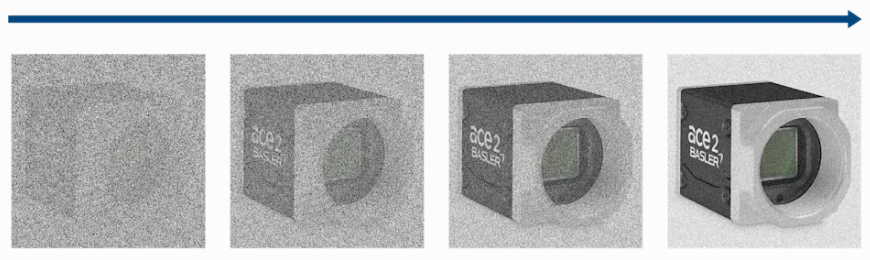
\includegraphics[width=1\linewidth]{Images/Week 2/snr.png}
    \caption{The signal-to-noise ratio: from low (left) to high (right) signal-to-noise ratio.}
\end{figure}
Once noise has become part of a signal, it can no longer be filtered or reduced. It is therefore advisable to take precautions to reduce the generation of noise, such as:
\begin{itemize}
    \item Use high-quality sensors and electronic devices in your camera.
    \item Use a good electronic architecture in the development of your camera.
    \item Lower the temperature of the sensor and other analog devices in your camera.
    \item Shield against interfering environmental conditions that affect the signal (e.g. by using shielded cables).
\end{itemize}
Camera users often increase the gain setting of their camera thinking that they are improving the signal-to-noise ratio. Since increasing the gain increases both the signal and the noise, the signal-to-noise ratio does not change significantly when the gain is increased. Gain is not an effective means of increasing the information content of the signal. Gain only changes the contrast of an existing image.

\subsection{Sensors}
\subsubsection{CCD}
A \textbf{charge-coupled device (CCD)} is an integrated circuit containing an array of linked, or coupled, capacitors. Under the control of an external circuit, each capacitor can transfer its electric charge to a neighbouring capacitor. CD sensors are a major technology used in digital imaging.
\begin{figure}[H]
    \centering
    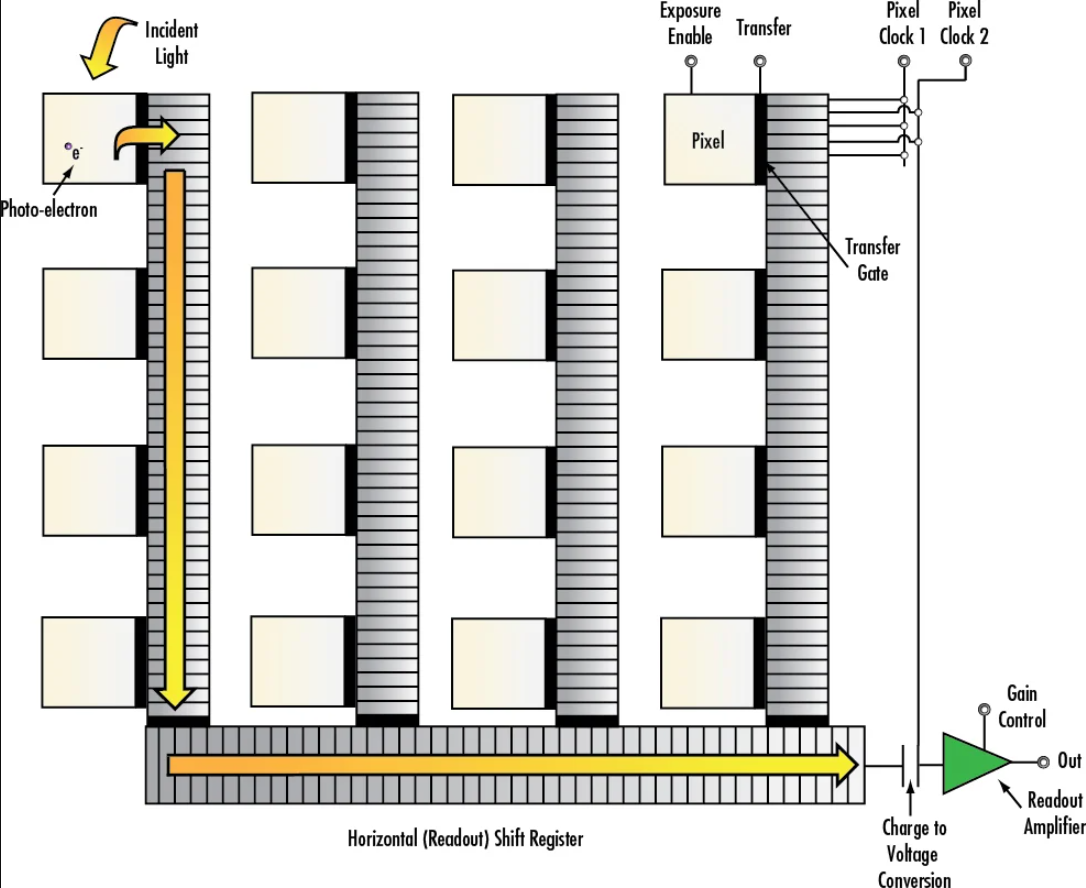
\includegraphics[width=1\linewidth]{Images/Week 2/ccd-schematic.png}
    \caption{Block Diagram of a Charge-Coupled Device (CCD).}
\end{figure}
In a CCD image sensor, pixels are represented by p-doped metal-oxide-semiconductor (MOS) capacitors. These MOS capacitors, the basic building blocks of a CCD, are biased above the threshold for inversion when image acquisition begins, allowing the conversoin of incoming photons into electron charges at the semiconductor-oxide interface; the CCD is then used to read out these charges.
Although they are not the only light-detection technology, they are widely used in applicaitons where high-quality image data are required.
\newline \newline
In a CCD for capturing images, there is a photoactive region (an epitaxial layer of silicon), and a transmission region made out of a shift register (the CCD). An image is projected through a lens onto the capacitor array, causing each capacitor to accumulate an electric charge proportional to the light intensity at that location.
A one-dimensional array, used in line-scan cameras, captures a single slice of the image, whereas a two-dimensional array, used in video and still cameras, captures two dimensional picture corresponding to the scene projected onto the focal plane of the sensor.
Once the array has been exposed to the image, a conrol circuit causes each capacitor to transfer its contents to its neighbour (operating as a shift register). The last capacitor in the array dumps its charge into a charge amplifier, which converts the charge into a voltage.
By repeating this process, the controlling circuit converts the entire contents of the array  in the semiconductor to a sequence of voltages. In a digital device, these voltages are then sampled, digitised, and usually stored in memory; in an analog device, they are processed into a continuous analog signal, which is then processed and fed out to other circuits for transmission, recording, or other processing.

\subsubsection{CMOS}
\textbf{Complementary metal-oxide-semiconductor (CMOS)} is an image sensor with an amplifier for each pixel, compared to the few amplifiers of a CCD. This results in less area for the capture of photons that a CCD, but this problem has been overcome by using microlenses in front of each photodiode, which focus light into the photodiode that would have otherwise hit the amplifier and not been detected. Some CMOS imaging sensors also used Back-side illumination to increase the umber of photons that hit the photodiode.
CMOS sensors can potentially be implemented with fewer components, use less power, and/or provide faster readout than CCD sensors. They are also less vulnerable to static electricity discharges.
\begin{figure}[H]
    \centering
    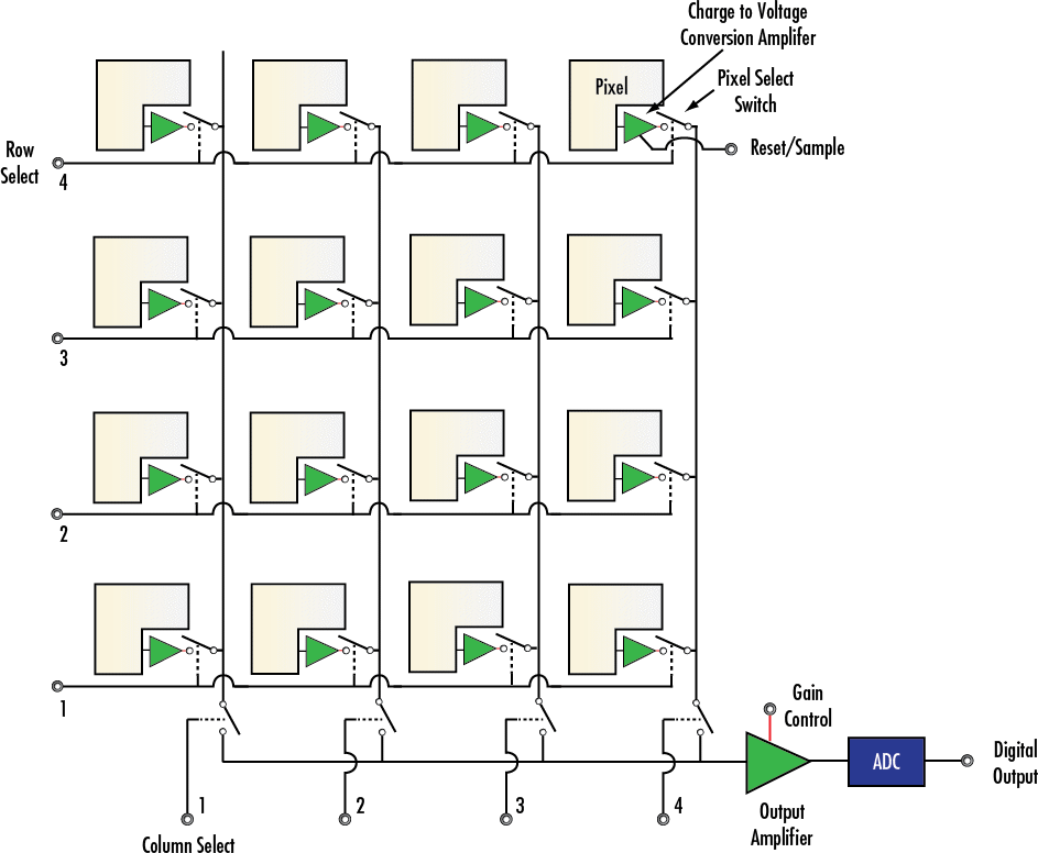
\includegraphics[width=1\linewidth]{Images/Week 2/cmos-schematic.png}
    \caption{Block Diagram of a Complementary Metal Oxide Semiconductor (CMOS).}
\end{figure}
\subsubsection{Performance}
There are many parameters that can be used to evaluate the performance of an image sensor, including dynamic range, SNR, and low-light sensitivity. For sensors of comparable types, the SNR and dynamic range improve as the size increases because in a given exposure time, more photons hit the pixel with larger area.

\subsubsection{Architecture}
CCDs converts incoming photos into electrons, which are then shifted across the sensor, pixel by pixel, to an output amplifier. The signal from each pixel is read out sequentially, one after another, leading to a slower readout process. CCDs traditionally offer higher sensitivity and lower noise due to the charge transfer process, amking them suitable for low-light conditions and scientific applications. Despite this, they generally consume more power and are most costly compared to CMOS sensors.
\newline \newline
In CMOS sensors, each pixel has its own amplifier and other circuitry, allowing for simultaneous readout of all pixels. The parallel readout enables much faster image capture compared to CCDs. They are typically cheaper and require less power to operate.
The presence of amplifiers and other circuitry can introduce more noise compared to CCDs.

\subsubsection{Shutter}
CCD sensors primarily use a global shutter, exposing the entire sensor at once, while CMOS sensors typically employ a rolling shutter, exposing the sensor line by line.
\newline \newline
The image from a CCD can result in more accurate representations of a single moment in time, minimising artifacts. If there's motion within the scene during the exposure, the global shutter can lead to a blurred image if the shutter speed is not fast enough to freeze the action.
In bright conditions, CCDs can be susceptible to vertical smear, where bright light overloads the sensor and spills into adjacent pixels.
\newline \newline
CMOS sensors typically expose the image line by line, creating a scan-like effect. This can lead to various motion artifacts like skew, wobble, and partial exposure.
CMOS sensors generally handle bright light better than CCDs and are less prone to blooming and smearing. In situations with flickering light sources, CMOS sensors may exhibit a rolling dark bar across the image.

\subsubsection{Overall Advantages vs. Disadvantages}
\textbf{CMOS - Advantages}:
\begin{itemize}
    \item \textbf{Lower power consumption}: Ideal for battery-powered devices.
    \item \textbf{Faster readout speeds}: CMOS sensors can capture and process images more quickly.
    \item \textbf{Lower manufacturing costs}: The simpler design and mass production capabilities of CMOS sensors make them cheaper to produce.
    \item \textbf{Greater flexibility and functionality}: They can be integrated with other features on the same chip, leading to more versatile and compact devices.
\end{itemize}
\textbf{CMOS - Disadvantages}:
\begin{itemize}
    \item \textbf{Higher noise levels}: The presence of amplifiers and ADCs at each piel can introduce more noise.
\end{itemize}

\textbf{CCD - Advantages}:
\begin{itemize}
    \item \textbf{Higher image quality in some applications}: CCD sensors were historically known for their ability to capture images with lower noise and better dynamic range, especially in scientific and astronomical imaging.
    \item \textbf{Softer, less digital-looking images}: Some users find the image rendering of CCD sensors to be more pleasing aesthetically, with a softer sharpness.
    \item \textbf{Low light sensitivity}: CCDs were known for good performance in low-light conditions.
\end{itemize}
\textbf{CCD - Disadvantages}:
\begin{itemize}
    \item \textbf{Slower readout speeds}: The sequential nature of signal transfer in CCDs can make them slower.
    \item \textbf{Larger size and complexity}: CCDs tend to be larger and more complex than CMOS sensors.
\end{itemize}
CMOS sensors have largely taken over the mainstream camera market due to their lower power consumption, faster speeds, and lower cost. CCD sensors are still used in specialised applications where their superior image quality in certain scenarios is crucial. 

\subsection{Pixel Architecture}
\subsubsection{Microlens}
A \textbf{microlens} is a small lens, with diameter less than a millimetre and often as small as 10$\mu$m. The samll sizes of the lenses means that a simple design can give good optical quality but sometimes unwanted effects arise due to optical diffraction at the samll features. A typical microlens may be a single element with one plane surface and one spherical convex surface to refract the light.
Because microlenses are so small, the substrate that supports them is usually thicker than the lens and this has to be taken into account in the design.
\newline \newline
A different type of microlens has two flat and parallel surfaces and the focusing action is obtained by a variation of refractive index across the lens. These are known as \textbf{gradient-index (GRIN) lenses}. Some micro-lenses achieve their focusing action by both a variation in refractive index and by the surface shape.
\newline \newline
Another class of microlens, sometimes known as \textbf{micro-Fresnel lenses}, focus light by refraction in a set of concentric curved surfaces. Such lenses can be made very thin and lightweight. Binary-optic micro-lenses focus light by diffraction. They have grooves with stepped edges or multilevels that approximate the ideal shape. They have advantages in fabrication and replication by using standard semiconductor processes such as photolithography and reactive-ion etching (RIE).
\newline \newline
Single micro-lenses are used to couple light to optical fibres; microlens arrays are often used to increase the light collection efficiency of CCD arrays and CMOS sensors, to collect and focus light that would have otherwise fallen onto the non-sensitive areas of the sensor.
\newline \newline
With optical sensor arrays, tiny lens systems serve to focus and concentrate the light onto the photo-diode surface, instead of allowing it to fall on non-photosensitive areas of the pixel device. Fill-factor is the ratio of the active refracting area, i.e. that area which directs light to the photo-sensor, to the total contiguous area occupied by the microlens array.

\subsubsection{Pixel Binning}
Pixel binning is a technique used in digital imaging where multiple adjacent pixels on a camera sensors are combined into a single, larger \textit{super pixel}. This process increases the SNR, especially in low-light conditions, by gathering more light photons to each super pixel. However, it reduces the resolution of the image since the number of pixels is decreased.
For example, a 2x2 binning operation combines the charge from four pixels into one.

\subsubsection{Back-side Illumination}
A \textbf{back-illuminated (BI) sensor},  also known as \textbf{back-side illumination (BSI)} sensor, is a type of digital image sensor that uses a novel arrangement of the imaging elements to increase the amount of light captured and thereby improve low-light performance.
\newline \newline
The technique was used for some time in specialized roles like low-light security cameras and astronomy sensors, but was complex to build and required further refinement to become widely used. Sony was the first to reduce these problems and their costs sufficiently to introduce a 5-megapixel 1.75$\mu$m BI CMOS sensor at general consumer prices in 2009.
BI sensors from OmniVision Technologies have since been used in consumer electronics from other manufacturers as in the HTC EVO 4G Android smartphone, and as a major selling point for the camera in Apple's iPhone 4.
\begin{figure}[H]
    \centering
    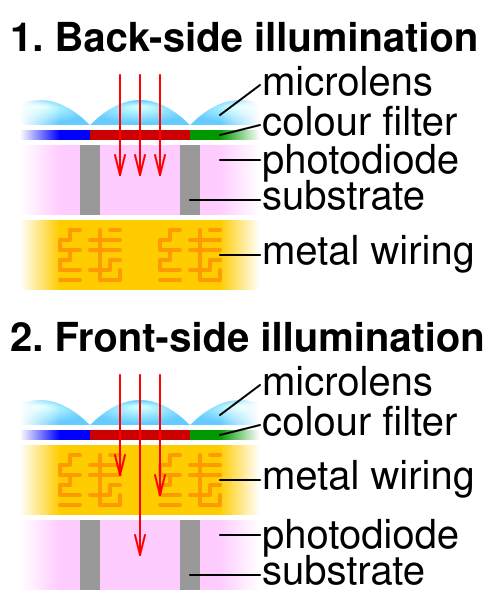
\includegraphics[width=1\linewidth]{Images/Week 2/Comparison_backside_illumination.png}
    \caption{Comparison of simplified back-illuminated and front-illuminated pixel cross-sections.}
\end{figure}
A traditional, front-illuminated digital camera is constructed in a fashion similar to the human eye, with a lens at the front and photodetectors at the back. This traditional orientation of the sensor places the active matrix of the digital camera image sensor, a matrix of individual picture elements, on its front surface and simplifies manufacturing. The matrix and its wiring, however, block some of the light, and thus the photocathode layer can only receive the remainder of the incoming light; the blockages reduces the signal that is available to be captured.
\newline \newline
A back-illuminated sensor contains the same elements, but arranges the wiring behind the photocathode layer by flipping the silicon wafer during manufacturing and then thinning its reverse side so that light can strike the photocathode layer without passing through the wiring layer.
This change can improve the chance of an input photon being captured from about 60\% to over 90\%, with the greatest difference realised when pixel size is small, as the light capture area gained in moving the wiring from the top (light incident) is proportionately larger for a smaller pixel.

\subsubsection{Resolution vs sensitivity trade-off}
The resolution vs sensitivity trade-off in CubeSat cameras is a fundamental optical and sensor design challenge.
\newline
Resolution is the level of detail a camera can capture. High resolution cameras use small pixels to fit more into an image. This increases the ability to distinguish small features.
\newline
Sensitivity is the ability to capture light. Low-light cameras, e.g., Sony A7S3, use larger pixels to capture more photons, increasing the SNR.
\newline
Since CubeSats have limited size for optics, restricted power and thermal budgets, and sometimes have extreme lighting conditions, it is important to find a balance between the two features.
Earth observation may prioritise resolution using higher quality optics and short exposure times (but may not work well on the dark side of Earth), whereas star tracking or imaging surfaces on the dark side of Earth would be better suited for a sensitive camera with slightly longer exposure times.
\newline \newline
To find a balance between the two and optimise the system, we can:
\begin{itemize}
    \item Use binning in dark areas to increase sensitivity when needed.
    \item Employ active exposure control or HDR techniques.
    \item Choose a sensor with back-illumination for better quantum efficiency.
    \item Use adaptive optics or onboard image enhancement.
\end{itemize}

\subsection{Analog Signal Processing}
\subsubsection{Signal Chain}
The camera sensor signal chain is a series of steps that convert photons into a digital image. It begins with the image sensor, where light is converted into an electrical signal, then amplified, filtered, and digitized before being processed and stored.
\begin{figure}[H]
    \centering
    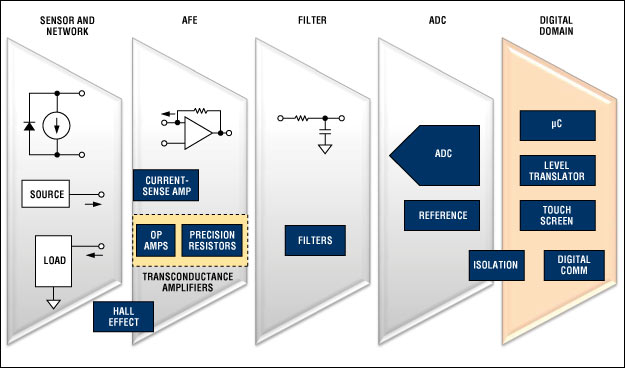
\includegraphics[width=1\linewidth]{Images/Week 2/photodiode-chain.jpg}
    \caption{Block diagram of camera sensor signal chain.}
\end{figure}
\begin{enumerate}
    \item \textbf{Image Sensor}: Light captured by the lens is focused on the image sensor, which contains millions of photodiodes.
    \item \textbf{Charge Conversion}: When light strikes a pixel, it generates a small electrical charge proportional to the light's intensity.
    \item \textbf{Signal Amplification}: The weak electrical signal from each pixel is amplified to improve its strength and signal-to-noise ratio.
    \item \textbf{Filtering}: Filters are used to remove unwanted noise and signals outside the desired frequency range. 
    \item \textbf{Analog-to-Digital Conversion (ADC)}: The amplified and filtered analog signal is converted into a digital signal by an ADC. This process samples the signal and assigns a digital value to each sample.
    \item \textbf{Image Processing}: The digital data then goes through further processing, including demosaicing (calculating the missing color information for each pixel), white balancing, sharpening, and noise reduction.
    \item \textbf{Storage}: Finally, the processed image data is stored on a memory card or transmitted to another device. 
\end{enumerate}
Different camera technologies, like CCD and CMOS sensors, have slightly different signal processing paths, but the core steps remain the same. For example, CCD sensors often require a more analog signal processing chain, while CMOS sensors have more integrated digital processing capabilities. 

\subsubsection{Noise Types}
In image sensors, common noise types include shot noise, read noise, and dark current noise. Shot noise arises from the statistical nature of photon detection, while read noise is introduced during the signal readout process. Dark current noise is caused by thermally generated electrons in the absence of light. These noise sources can significantly impact image quality, especially in low-light conditions or with long exposures. 
\newline \newline
\textbf{Shot noise}, also known as photon noise, is a fundamental noise source caused by the inherent randomness in the arrival of photons at the image sensor.
Photons, being discrete particles, don't arrive at a perfectly uniform rate, leading to fluctuations in the number of detected electrons.  Shot noise is signal-dependent, meaning it increases with the strength of the incoming light signal. 
In high-light conditions, shot noise becomes the dominant noise source, while in low-light conditions, other noise sources might be more significant. 
\newline \newline
\textbf{Read noise}, is introduced during the process of converting the electrical signal from the sensor into a digital value. It originates from the electronic components within the camera, such as amplifiers and analog-to-digital converters.
Read noise is generally independent of the signal level and sensor temperature. Read noise is often the dominant noise source in low-light or short-exposure images.
\newline \newline
\textbf{Dark current noise}  is a small electrical current that flows in a sensor even when no light is detected. It is primarily caused by thermal generation of electrons within the sensor material.
Dark current increases with temperature and exposure time. Dark current noise can be a significant issue in long-exposure images or when using high-sensitivity sensors. 
\newline \newline
\textbf{Fixed pattern noise (FPN)} is a type of noise in digital imaging sensors characterised by a consistent, repeating pattern across the image. It arises from manufacturing variations in the sensor, leading to some pixels having slightly different responses than others, regardless of the scene being captured. This pattern remains the same in each image, making it distinct from random noise. FPN is often more noticeable in low-light or long-exposure images. 
\newline \newline
\textbf{Quantisation noise} is the error introduced when a continuous analog signal is converted into a discrete digital signal. This happens because the digital system can only represent a finite number of levels, so the original signal is rounded to the nearest available level. This rounding process creates a difference between the original and the quantized signal, which is perceived as noise. 
\newline \newline
\textbf{Thermal or Johnson-Nyquist noise} , is the random voltage or current noise generated by the thermal agitation of charge carriers (like electrons) within electrical conductors at equilibrium, regardless of any applied voltage. It's a fundamental noise source present in all electrical circuits and is proportional to the absolute temperature. This noise can limit the sensitivity of sensitive electronic equipment, such as radio receivers, and is particularly noticeable at low signal levels. 
\newline \newline
For a slightly more in-depth explanation of the different noise types, this \href{https://www.thorlabs.com/newgrouppage9.cfm?objectgroup_id=10773}{source} dives into more detail. In cameras, noise reduces the SNR, which makes it harder to detect real features in an image. This is especially problematic in low-light conditions, where the signal is weak and noise may dominate.
High noise floors limit the minimum detectable signal. It also compresses the dynamic range, making it harder to distinguish between bright and dark regions in a scene.
Noise characteristics will influence the choice of  the sensor and pixel size, gain settings, ADC resolution, and the need for cooling, shielfing, or post-processing corrections (like dark frame subtraction and/or denoising).


\subsection{Sensor Control Interfaces}
\label{sec:sony-imx}
Here, we will investigate the basics of the \textbf{Sony IMX219PQH5-C} image sensor, found \href{https://www.opensourceinstruments.com/Electronics/Data/IMX219PQ.pdf}{here}.
\newline \newline
\subsubsection{Overview}
The IMX219PQH5-C is a diagonal 4.60 mm (Type 1/4.0) CMOS active pixel type image sensor with a square pixel array and 8.08M effective pixels. This chip operates with three power supplies, analogue 2.8 V, digital 1.2 V, and IF 1.8 V, and has low power consumption. High sensitivity, low dark current, and no smear are achieved through the adoption of R, G, and B primary color pigment mosaic filters. This chip features an electronic shutter with variable charge-storage time.
\begin{figure}[H]
    \centering
    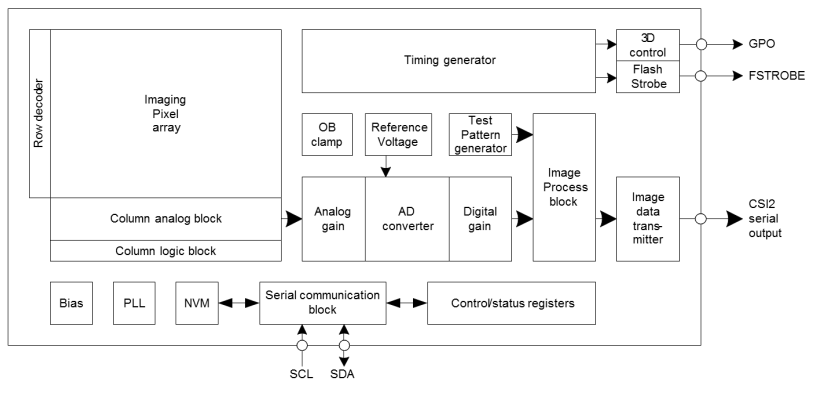
\includegraphics[width=1\linewidth]{Images/Week 2/sony-imx.png}
    \caption{Overview of functional block diagram.}
\end{figure}

\subsubsection{Features}
\begin{itemize}
    \item Back-illuminated CMOS image sensor (Exmor R\texttrademark)
    \item On-chip 2-wire serial communication interface
    \item MIPI CSI-2 data output (2 or 4 lanes selectable)
    \item Integrated timing generator and horizontal/vertical driver circuits
    \item On-chip CDS (Correlated Double Sampling) and PGA (Programmable Gain Amplifier)
    \item 10-bit on-chip A/D conversion
    \item On-chip automatic optical black (OB) clamp circuit
    \item On-chip PLL (rectangular wave)
    \item High sensitivity, low dark current, no smear
    \item Strong anti-blooming performance
    \item Variable-speed shutter (1 H step)
    \item RGB primary color pigment mosaic filter
    \item Max 30 fps in full-resolution (all-pixel scan) mode
    \item Pixel rate: 280 Mpixel/s in all-pixels mode
    \item High-speed modes: 
        \begin{itemize}
        \item 180 fps @720p with 2*2 analog binning
        \item 60 fps @1080p with vertical cropping
        \end{itemize}
    \item Data rate: up to 755 Mbps/lane (4-lane), 912 Mbps/lane (2-lane)
\end{itemize}

\subsubsection{Communication Protocol}
This sensor uses the 2-wire serial communication method for sensor control. These specifications are described for sensor control using the 2-wire serial communication as follows.
\begin{figure}[H]
    \centering
    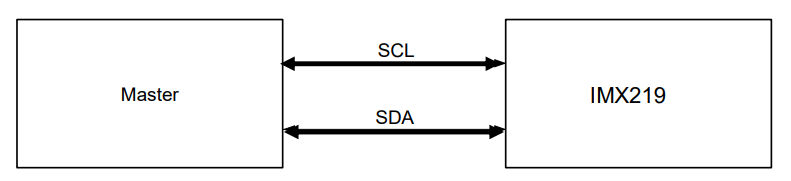
\includegraphics[width=1\linewidth]{Images/Week 2/sony-imx-wire.png}
    \caption{2-wire serial communication.}
\end{figure}
The 2-wire serial communication method conforms to the Camera Control Instance (CCI). CCI is an I$^2$C fast-mode compatible interface, and the data transfer protocol is the I$^2$C standard. This 2-wire serial communication circuit can be used to access the control registers and status-registers of this sensor.
\newline \newline
2-wire serial communication supports a 16-bit register address and 8-bit data message type.
\begin{figure}[H]
    \centering
    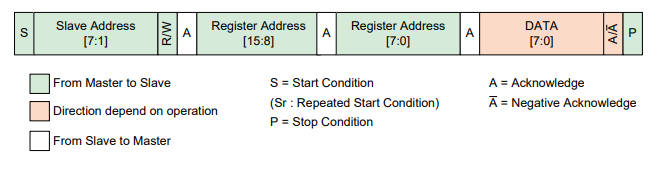
\includegraphics[width=1\linewidth]{Images/Week 2/2-wire-protocol.png}
    \caption{2-wire serial communication protocol.}
\end{figure}

\subsubsection{Register Control}
Naturally, all the register controls cannot be listed on a single page since most drivers for these types of image sensors are thousands of lines long. For simplicity, we will cover a few examples of setting up the registers for a specific purpose.
\newline \newline
\textbf{Analog gain} on the sensor can be set using the following equation:
\[
G=\frac{m0\times X+c0}{m1\times X + c1}
\]
The variables are shown in the table below.
\begin{figure}[H]
    \centering
    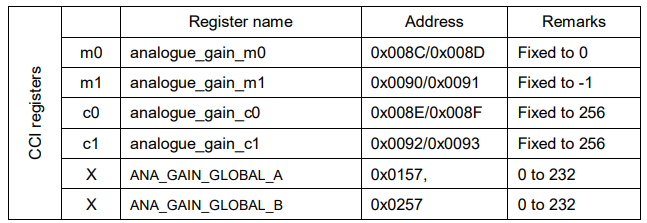
\includegraphics[width=1\linewidth]{Images/Week 2/gain-table.png}
    \caption{Gain setting variables.}
\end{figure}
Therefore, the analogue gain is as follows:
\[
G = \frac{256}{256-X}
\]
Where $X$ can be controlled between 0-232 via the 0x0157 or 0x0257 register address.
\newline \newline
The default \textbf{readout position} is from the lower left corner when Pin 1 is located in the upper right corner. The image is inverted vertically and horizontally by the lens, so proper output results when Pin 1 is located in the upper right corner.
\begin{figure}[H]
    \centering
    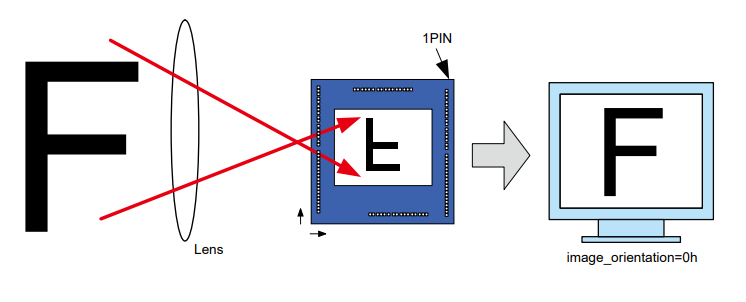
\includegraphics[width=1\linewidth]{Images/Week 2/readout-pos.png}
    \caption{Readout Position.}
\end{figure}
Readout direction can be set by the registers:
\begin{figure}[H]
    \centering
    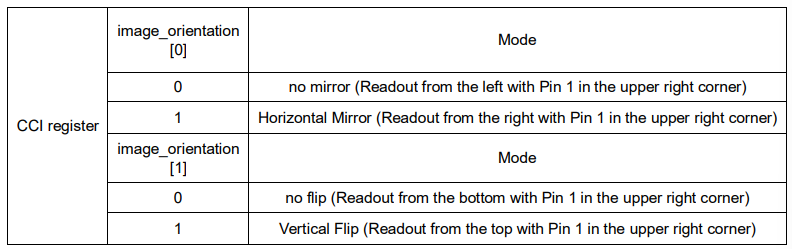
\includegraphics[width=1\linewidth]{Images/Week 2/readout-table.png}
    \caption{Image Orientation Register.}
\end{figure}
\begin{figure}[H]
    \centering
    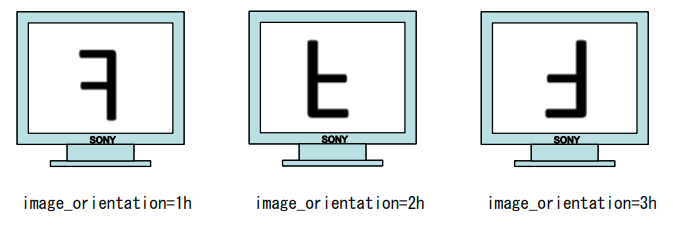
\includegraphics[width=1\linewidth]{Images/Week 2/vh-mirror.png}
    \caption{Output Image Diagrams for Vertical Flip and Horizontal Mirror.}
\end{figure}

The \textbf{temperature sensor} measures the junction temperature of the silicon sensor. The target range is -10 to 95\textdegree C, with $\pm5$\textdegree in deviation. The sensor is operated immediately after streaming mode, and the value will be stored in the register.
\newline
Registers to be related about temperature sensor are the followings:
\begin{figure}[H]
    \centering
    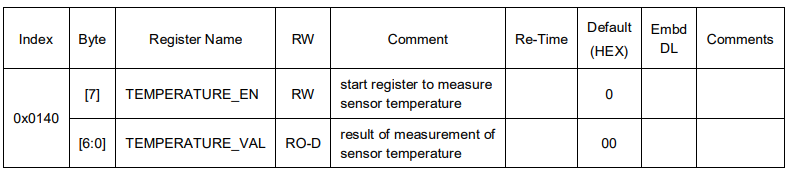
\includegraphics[width=1\linewidth]{Images/Week 2/temp-register.png}
    \caption{Temperature setting registers.}
\end{figure}
The following table shows the relationship between temperature and stored value:
\begin{figure}[H]
    \centering
    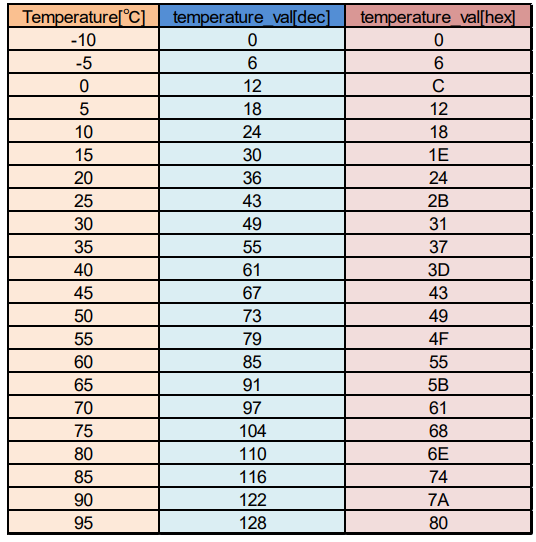
\includegraphics[width=1\linewidth]{Images/Week 2/temp-table.png}
    \caption{Temperature value relationship.}
\end{figure}


% -----------------------
% WEEK 3
% -----------------------

\section{Image Processing Pipeline}

\subsection{Demosaicing and Bayer pattern reconstruction}
\textbf{Demosaicing}, also known as colour reconstruction, is a digital image processing algorithms used to reconstruct a full colour image from the incomplete samples output from an image sensor averlaid with a colour filter array like a Bayer filter. It is also known as CFA interpolation or debayering.
\newline \newline
Most modern digital cameras acquire images using a single image sensor overlaid with a CFA, so demosaicing is part of the processing pipeline required to render these images into a viewable format. Many modern cameras can save images into a .RAW format, allowing the user to demosaic them using software, rather than using the camera's built-in firmware.
\newline \newline
The aim of a demosaicing algorithm is to reconstruct a full colour image from the spatialy undersampled colour channels output from the CFA. The algorithm should have the following traits:
\begin{itemize}
    \item Avoidance of the introduction of false colour artifacts, such as chromatic aliases, zippering and purple fringing
    \item Maximum preservation of the image resolution
    \item Low computational complexity for fast processing or efficient in-camera hardware implementation
    \item Amenability to analysis for accurate noise reduction
\end{itemize}

\subsubsection{Bilinear vs edge-aware algorithms}
Bilinear and edge-aware demosaicing are two different approaches to reconstructing a full-colour image from a Bayer filter mosaic.
\newline \newline
\textbf{Bilinear interpolation} is a simple, fast method that averages neighbouring pixel values to estimate missing colour components, but it often produces artifacts, especially around edges.
\newline \newline
\textbf{Edge-aware algorithms}, on the other hand, are more sophisticated, taking into accound image edges and high-frequency details to produce a more accurate reconstruction.

\subsection{White Balance, Gamma, and Exposure Control}
\subsubsection{White Balance}
\textbf{White balance} is a camera setting that adjusts colours in an image to make white objects appear white, regardless of the colour temperature of the light source. It ensures photos are depicted accurately by compensating for the colour cast of different light sources light sunlight or artificial light.
While white balance specifically targets whites, white balance affects all colours in the image because it adjusts the overally colour temperature.
\newline \newline
Colour temperature is measured in Kelvin (K) and describes the relative warmth or coolness of white light. Lower temperatures (e.g., 2700K) represent warmer, reddish-yellow light (like incandescent bulbs).
Higher temperatures represent cooler, bluish light (like fluorescent lights).
\newline \newline
Whilst you can acheive white balance in post-processing, it's often best to get it as close as possible in-camera for the best results, especially when shooting in .RAW format.
\newline \newline
Depending on the orbit or target, we may face different lighting conditions (e.g., reflected sunlight, albedo changes) that will impact the image. If the white balance is not correct and we do not shoot in .RAW, the colour data is most likely unrecoverable. Many sensors like the IMX477 include auto-WB; but for scientific data, manual tuning or calibrated WB is often better.

\subsubsection{Gamma Correction}
\textbf{Gamma correction} or \textbf{gamma} is a nonlinear operation used to encode and decode luminance or tristimulus values in video or still image systems. Gamma correction is, in the simplest cases, defined by the following power-law expression \(V_{out}=AV_{in}^{\gamma}\),
where the non-negative real input value $V_{in}$ is raised to the power of $\gamma$ and multiplied by the constant $A$ to get the output value $V_{out}$. In the common case of $A=1$, inputs and outputs are typically in the range of 0-1.
\newline \newline
A gamma value $\gamma<1$ is sometimes called an encoding gamma, and the process of encoding with this compressive power-law nonlinearity is called \textbf{gamma compression}; conversely, a gamma value $\gamma>1$ is called \textbf{decoding gamma}, and the expansive power-law nonlinearity is called \textbf{gamma expansion}.
\begin{figure}[H]
    \centering
    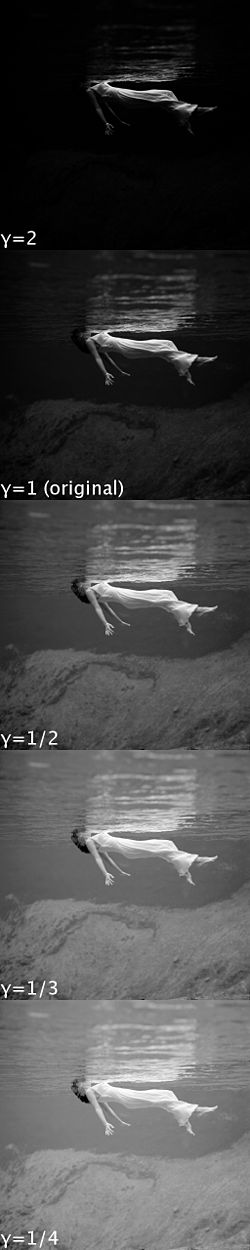
\includegraphics[width=0.35\linewidth]{Images/Week 3/gamma-ex.jpg}
    \caption{The effect of gamma correction on an image: the original image was taken to varying powers, showing that powers larger than 1 make the shadows darker, while powers smaller than 1 make dark regions lighter. This is not the actual gamma the picture has, though.}
\end{figure}
Digital cameras record light using electronic sensors that usually respond linearly. In the process of rendering linear raw data to conventional RGB data (e.g. for storage into JPEG image format), color space transformations and rendering transformations will be performed.
In particular, almost all standard RGB color spaces and file formats use a non-linear encoding (a gamma compression) of the intended intensities of the primary colors of the photographic reproduction. In addition, the intended reproduction is almost always nonlinearly related to the measured scene intensities, via a tone reproduction nonlinearity.
\newline \newline
For the CubeSat, since the imagery will most likely be used for Marketing i.e., human interpretation, gamma correction improves perceived contrast and dynamic range. Applying gamam before compression (e.g., JPEG, H.264) often improves results since gamma-adjusted images compress better visually.

\subsubsection{Exposure Control}
\textbf{Exposure} is the amount of light per unit area reaching a frame of an electronic image sensor. It is determined by the shutter speed, lens f-number, and scene luminance. Exposure is measured in units of lux-seconds (lx$\cdot$s) and can be computed from exposure value (EV) and scene luminance in a specified region.
\newline \newline
\textbf{Radiance exposure} of a surface, denoted $H_e$ ("e" for energetic) and measured in J/m$^2$, is given by $H_e=E_et$, where:
\begin{itemize}
    \item $E_e$ is the irradiance of the surface, measured in W/m$^2$;
    \item $t$ is the exposure duration, measured in s.
\end{itemize}
\textbf{Luminous exposure} of a surface, denoted $H_v$ ("v" for visual) and measured in (lx$\cdot$s), is given by $H_v=E_vt$, where:
\begin{itemize}
    \item $E_v$ is the illuminance of the surface measured in lx;
    \item $t$ is the exposure duration, measured in s.
\end{itemize}
For the CubeSat, clouds, city lights, terrain albedo, or planetary bodies all vary in brightness so it is important to develop a system to maintain consistency between images so data isn't lost between images (saturation).

\subsection{Noise Reduction and Sharpening}
Spatial noise in imaging is the variations or irregularities in the pixel values of an image that are unrelated to the actual features of the scene being captured. This type of noise occurs at the pixel level and can introduce unwanted randomness or fluctuations in the visual information.
\newline \newline
Spatial noise majorly occurs due to sensor imperfections. The individual pixels in a sensor vary from each other in terms of the sensitivity of minor defects. This leads to spatial noise in the image captured.
\newline \newline
There are also various other sources of spatial noise. External environmental factors such as temperature difference, electromagnetic interference, and vibration can also introduce spatial noise into the imaging system. Spatial noise can also occur during the digitization process when the continuous range of analog signal values is converted into discrete digital values. This leads to quantisation errors and, in turn, gives rise to quantisation noise.
\subsubsection{Convolutions}
Convolution is a formal mathematical operation used in image processing applications. The different types of noise reduction methods in the following section are done using convolution operation.
\newline \newline
Convolution is done using a small matrix called a kernel or filter comprised of integers. Differently sized kernels containing different patterns of numbers produce different results under convolution. The size of the kernel is arbitrary, but 3×3 is used more often. The anchor point in the kernel is used to know the position of the kernel with respect to the image.
\begin{figure}[H]
    \centering
    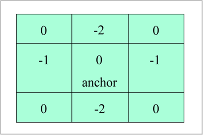
\includegraphics[width=0.7\linewidth]{Images/Week 3/kernel.png}
    \caption{Kernel or Filter}
\end{figure}
The kernel is slid or convolved across the entire image. The positioning of the kernel on top of the image pixel starts from the top left corner. And it is moved sequentially till the end. At each position, the element-wise multiplication of the kernel and the underlying image patch is computed. This is followed by summing up these products to obtain the value for the corresponding pixel in the output image.
\[
(I\star K)(x,y)=\sum_i \sum_j I(x+i, y+j)\cdot K(-i, -j)
\]
Alternatively for continuous domains, the convolution is expressed using an integral rather than a sum.
\[
(I\star K)(x,y)=\int \int_{-\infty}^{\infty} I(u,v)\cdot K(x-u,y-v)dudv
\]
However, in practice images are discrete, so only the former is used. In theory, we idealise images as continuous functions for image analysis and physics-based modelling since the real world is continuous and cameras turn the continuous data into discrete packets.

\subsubsection{Average Smoothing}
In average smoothing, the intensity difference between pixel-to-pixel (i.e., the noise in the image) is reduced by an averaging technique. The kernel/matrix used in average smoothing is shown below.
\begin{figure}[H]
    \centering
    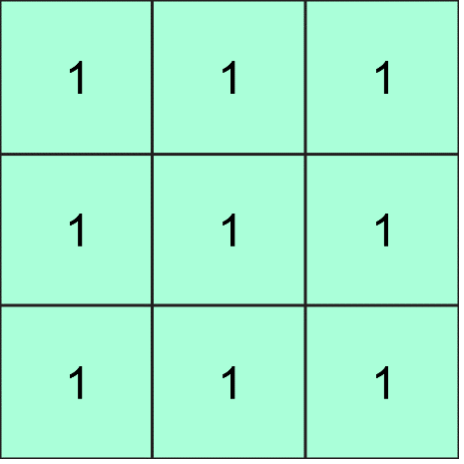
\includegraphics[width=0.7\linewidth]{Images/Week 3/average-kernel.png}
    \caption{Kernel Used in Average Smoothing}
\end{figure}
In average smoothing, the kernel window used is a square matrix with equal weights. It is usually a square matrix of size (n x n), where 'n' is an odd number. The 'n' being odd is to have a well-defined, symmetric neighborhood around each data point. The above given (Figure 2) matrix is a 3×3 kernel, with the weights evenly distributed.
\newline \newline
The kernel window will be placed above the image pixel being processed (i.e., slide the kernel across each data point in the image). The average of the data points in the image matrix under the kernel window is calculated. The current data point in the image pixel is replaced with the calculated average. This process is repeated for every data point in the image.
\begin{figure}[H]
    \centering
    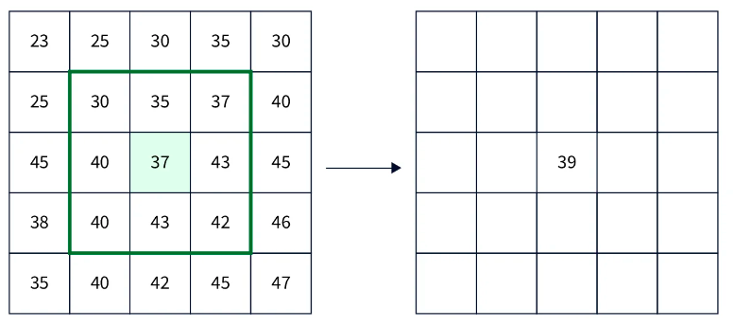
\includegraphics[width=1\linewidth]{Images/Week 3/average-ex.png}
    \caption{Average Smoothing Example}
\end{figure}

\subsubsection{Gaussian Filter}
Gaussian filter is a spatial noise reduction method used for reducing high-frequency noise. This filtering technique uses the Gaussian function to perform convolution.
\newline \newline
The difference between the Gaussian filtering technique and average smoothing is that, in Gaussian filtering, more weight values are assigned to the points closer to the center pixels, and lesser weight values are assigned to points far away from the center pixel. This results in a smoother transition. This varying weight distribution allows the Gaussian filter to reduce noise effectively while preserving important details in the image.
\begin{figure}[H]
    \centering
    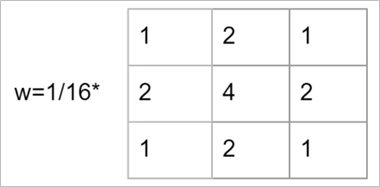
\includegraphics[width=0.7\linewidth]{Images/Week 3/gauss-kernel.png}
    \caption{Example of Gaussian Filter Kernel with Standard Deviation of 1}
\end{figure}
In the above example, the standard deviation is assumed to be 1. The values in the matrix are the weights assigned to the neighboring pixels during the convolution operation. The central pixel has the highest weight, and the weights decrease as we move away from the center.

\subsubsection{Median Filter}
The Median filtering technique is commonly used for removing salt-and-pepper noise. It is widely used in the medical field as this kind of noise is prevalent in medical imaging.
\newline \newline
Just as in other filtering techniques discussed above, in a Median filter, a kernel matrix is slid over the entire image. Move the selected window over each pixel in the image, covering one pixel at a time. For each window placement, collect the pixel values within the window and sort them in ascending order. The median is the middle value in the sorted list. Assign the median value as the new value for the pixel at the center of the window. This process is repeated for every pixel in the image.
\begin{figure}[H]
    \centering
    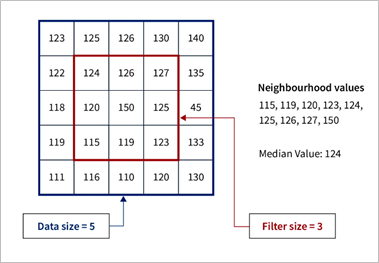
\includegraphics[width=0.7\linewidth]{Images/Week 3/mediabn-kernel.png}
    \caption{Median Filtering Example}
\end{figure}
The key advantage of median filtering is its ability to effectively remove salt-and-pepper noise (random bright and dark pixels) in an image without significantly blurring edges. Since the median is less sensitive to extreme values than the mean, it tends to preserve edges and details in the image.

\subsubsection{Bilateral Filter}
Bilateral filtering is a non-linear, edge-preserving noise filtering technique. It is particularly effective in smoothing images while preserving edges. The filter takes into account both the spatial distance between pixels and the intensity differences, allowing it to retain important image features while reducing noise.
\newline \newline
Bilateral filtering does not blur the images too much because it considers both how far pixels are from each other and how different their colors are. This helps preserve the important details, like edges in the image.

\subsubsection{Nonlocal Means}
Non-local Means (NLM) is a technique used in image denoising, aiming to reduce noise while preserving image details. Unlike traditional denoising methods, which operate locally on each pixel or small neighborhood, non-local means consider similarities across the entire image for better noise reduction. The NLM does not use the convolution technique to do the filtering but uses the NLM algorithm.
The non-local means technique leverages the idea that similar structures in an image should have similar noise characteristics. By final output image's non-local similarities, the algorithm can effectively distinguish between signal and noise, leading to improved denoising performance.

\subsubsection{Weiner Filter}
The Wiener filter assumes that the given image is a combination of a true underlying image (signal) and additive noise. The Wiener filter calculates the Power Spectral Density (PSD) of both the signal (the true image) and the noise. The PSD provides information about how the energy is distributed across different frequencies in the signal and the noise. It considers the Signal-to-Noise Ratio (SNR), which is a measure of how strong the signal is compared to the noise. A high SNR means a strong signal and less noticeable noise.
\newline \newline
Using the information from the PSD and SNR, the Wiener filter creates a filter function. This function is designed to attenuate (reduce) frequencies dominated by noise while preserving frequencies dominated by the signal. The filter adapts its behavior based on the characteristics of the signal and noise.
\newline \newline
In simpler terms, the Wiener filter is like a smart cleaner for images that understands which parts of the image are important (signal) and which parts are unwanted noise. It then applies a special filter to keep the important stuff while reducing the noise, resulting in a clearer and cleaner image. The key is adapting the filter based on the statistical properties of the signal and noise, making it a powerful tool for image denoising.
\begin{figure}[H]
    \centering
    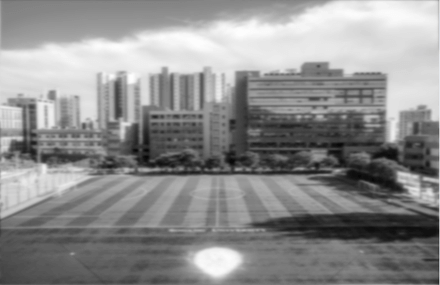
\includegraphics[width=1\linewidth]{Images/Week 3/weiner-ex.png}
    \caption{Before and After Images of Weiner Filter}
\end{figure}

\subsubsection{Sharpness vs. Artifacts}
In image processing, there's often a trade-off between sharpness and artifacts. Increasing sharpness can enhance details but may also introduce or amplify undesirable visual artifacts like noise, halos or ringing. Conversely, reducing sharpening can mitigate these artifacts but may results in a softer, less detailed image.
\newline
It is difficult to decide what balance between sharpness and artifacts the CubeSat camera will require currently, so it is important to test parameters to determine the best balance.

\subsection{Colour Space and Conversion}
\subsubsection{RGB}
\textbf{RGB colour spaces} are a category of additive colourimetric colour spaces specifying part of its absolute colour space definition using the RGB colour model.
\newline \newline
RGB colour space are commonly found describing the mapping of the RGB colour model to human perceivable colour, but some RGB colour spaces use imaginary (non-real-world) primaries and thus cannot be displayed directly.
\newline \newline
The normal human eye contains three types of color-sensitive cone cells. Each cell is responsive to light of either long, medium or short wavelengths, which we generally catergorise as red, green and blue. Taken together, the responses of these cone cells are called the \textbf{tristimulus values} and the combination of their responses is processed into the psychological effect of colour vision.
RGB use in color space definitions employ primaries (and often a white point) based on the RGB color model, to map to real world color. Applying Grassmann's law of light additivity, the range of colors that can be produced are those enclosed within the triangle on the chromaticity diagram defined using the primaries as vertices.
\newline \newline
RGB color spaces are well-suited to describing the electronic display of color, such as computer monitors and color television. These devices often reproduce colours using an array of red, green, and blue phosphors agitated by a cathode-ray tube (CRT), or an array of red, green, and blue LCDs lit by a backlight, and are therefore naturally described by an additive color model with RGB primaries.
It also directly maps to the output of Bayer filters on image sensors where each pixel stores a red, green and blue value, however, they are not optimal for compression.

\subsubsection{Y'UV}
\textbf{Y'UV}, also written \textbf{YUV}, is the colour model found in the PAL analogue colour TV standard. A colour is described as a Y' component (luma) and two chroma components (U and V). The prime symbol denotes that the luma is calculated from gamma-corrected RGB input and that it is different from the true luminance.
Today, the term YUV is commonly used in the computer industry to describe colorspaces that are encoded using YCbCr.
\newline \newline
An advantage of Y'UV is that some of the information can be discarded in order to reduce bandwidth. The human eye has fairly little spatial sensitivity to color: the accuracy of the brightness information of the luminance channel has far more impact on the image detail discerned than that of the other two. Understanding this human shortcoming, standards such as NTSC and PAL reduce the bandwidth of the chrominance channels considerably. (Bandwidth is in the temporal domain, but this translates into the spatial domain as the image is scanned out.)
\newline \newline
This colour space is efficient for data storage and transmission but not for .RAW image capturing or sensor processing. It usually requries a conversion from RGB (which is an extra computation step).

\subsubsection{HSV}
\textbf{HSL} and \textbf{HSV} are the two most common cylindrical-coordinate representations of points in an RGB model. The two representations rearrange the geometry of RGB in an attempt to be more intuitive and perceptually relevant than the cartesian representation. Developed in the 1970s for computer graphics applications, HSL and HSV are used today in color pickers, in image editing software, and less commonly in image analysis and computer vision.
\newline \newline
HSV is rarely used directly for capture or compression. It is useful for onboard vision algorithms like object detection and segmentation, but not efficient for storage or transmission, and like Y'UV, must be converted from RGB.

\subsubsection{Chroma Subsampling}
Chroma subsampling is a technique used in digital image and video compression where the color information (chroma) is stored at a lower resolution than the luminance (brightness) information.
This takes advantage of the human visual system's lower sensitivity to color details compared to brightness. By reducing the amount of color data, chroma subsampling can significantly reduce file sizes and bandwidth requirements without a major perceived loss in image quality.
Since Y'UV stores its luminance and chroma differently, it is much better for chroma subsampling / compression.
\newline \newline
Although modern display devices don't all work this way, the concept of scanlines is still important because chroma subsampling types are specified horizontally. Each type is often listed as a ratio between the rate at which luma and chroma values are sent as a line is scanned. This ratio is typically based on four luma values, and takes the form 4:X:Y, where X and Y are the relative number of chroma values for in rows of a conceptual 4x2 pixel block.
\newline \newline
Using the standard nomenclature, 4:2:2 means each horizontal scanline has 2 chroma values for every 4 luma values. Similarly, 4:1:1 means 1 chroma value is sent for every 4 luma values sent, and 4:4:4 means no chroma subsampling. However, this is not entirely consistent. 4:2:0 would imply that for every 4 luma values, there would be 2 for the first chroma component and 0 for the second but this wouldn't produce full color images. In practice, 4:2:0 instead means there are two of each chroma sample per scanline, but that these are only present every other line.
\newline \newline
Check out \href{https://www.red.com/red-101/video-chroma-subsampling#:~:text=Using%20the%20standard%20nomenclature%2C%204:2:2%20means%20each,subsampling.%20However%2C%20this%20is%20not%20entirely%20consistent.}{this site} for visual examples of how chroma subsampling works and its impact quality.
\newline \newline
Although chroma subsampling has been an easy yet effective compression technique since the early days of video, it can create noticeable artifacts. Digital techniques have also become far more sophisticated since then.
Whereas subsampling utilises a simple image-wide reduction in color resolution, modern digital codecs can analyse image content and decide how to prioritise that detail. Regions with lower brightness, less saturation and coarser detail can all be treated differently with digital.

\subsection{Image Compression and File Formats}

\subsubsection{Lossy vs. Lossless for Space Applications}
It is important to know the concept of lossy and lossless file compression. A \textbf{lossy algorithm} removes some information in the digital file to reduce the file size. However, the loss of information lowers the overall quality of the image. Lossy files can be saved in your computer at various quality levels.
On the other hand, a \textbf{lossless algorithm} retains all the information in the image. But that also means lossless files takes a lot of space in your storage device.
\newline \newline
In space applications, the choice between lossless and lossy compression depends on the specific data and the priorities of the mission.
Lossless compression is preferred for critical data where no information can be lost, such as scientific measurements or control parameters. Lossy compression is suitable for less critical data like images or videos where some data loss is acceptable for achieving higher compression ratios and reduced storage and transmission needs.
\newline \newline
If the data is critical and cannot tolerate any loss of information, lossless compression is the only option.
If storage space and bandwidth are limited, lossy compression can be used for non-critical data to reduce file sizes and transmission time. Lossy compression offers higher compression ratios, but it's important to evaluate the impact of data loss on the application.

\subsubsection{RAW}
RAW files are processed directly from the camera's sensor, thus they do not use compression. Because they are lossless, the images are extremely high-quality. They show more shades of colors and better representation of white balance, contrast, exposure  etc. In addition, changes made to RAW files are non-destructive. Only the metadata that controls the rendering is altered, but the original file data remains untouched.
\newline \newline
Obviously, fewer images can be saved in your memory card or hard drive due to the massive amount of data in the RAW file. Also, there is no widespread adoption of a standard RAW format.
As such, specialised software may be needed to open RAW files. However, this drawback has been mitigated by using open-source computer programs such as dcraw.
\newline \newline
Many photographers, editors, and graphic artists use RAW images during the editing phase. However, they usually save the final result in a more compressed format (most likely JPEG).

\subsubsection{DNG}
DNG is a lossless format similar to RAW. However, unlike RAW that uses specific formats based on camera types or manufacturers, DNG stores image data in a compatible, generic format. Thus, even if it is created by Adobe for its applications, any software that can read or convert DNG format can be used.
\newline \newline
Converting RAW files to DNG is highly recommended as this will significantly decrease the size of the images, making them easy to download, upload, or send via email. In fact, DNG files are 15 to 20 percent smaller in size than RAW files without any loss of quality.
\newline \newline
The DNG format has checksum information that is used to scan and prevent file corruption. Also, enhancements, new features, and extra functionalities are assured since Adobe continuously works on the DNG format.
\newline \newline
However, it takes a long time to convert RAW files into DNG. The format also removes unrecognised metadata from RAW files, making it virtually impossible to retrieve such data from DNG files in the future. Finally, since any alteration is written directly into the DNG file, you have to back up the entire file each time a change is made.

\subsubsection{GIF}
GIF, Graphics Interchange Format, is great for graphics and animations. Web designers and graphic artists ofen use them because extreme data compression considerably decreases the size of GIF files allowing them to quickly load, however, this makes it not recommended for photos/photography.

\subsubsection{PNG}
PNG, Portable Network Graphic, originally created as an improved replacement for GIF, is a popular format used by photographers and graphic designers. That's because the format supports lossless data compression, which means a lot of information is retained when you save and reopen your images.
\newline \newline 
There is data compression involved but not as much as in GIFs, which allows you to retain a high-quality image. However, the size, although compressed, is still more than a JPEG image.

\subsubsection{JPEG}
Used by most digital cameras as their default format, JPEG, Joint Photographic Experts Group, is the most common file type which can be used online or for hard prints.
Its lossy compression algorithm removes minute details that your eye is least likely to notice to save space. However, the compression ratio is adjustable so you can select the level of quality you want in your image. In general, the compression is enough to provide a reasonably high-quality image without worrying too much about the file size.
\newline \newline 
JPEG is chosen as the preferred file format for CubeSat image transmission due to its balance of image quality and compression.
CubeSats often operate with limited bandwidth, so reducing file size is essential.
JPEG uses lossy compression to remove visual data that is less noticeable to the human eye, making it well-suited for efficient transmission.
The compression level is adjustable, allowing operators to prioritise either image quality or file size based on mission needs.
Baseline JPEG is typically used because it is widely supported and simple to decode on ground stations.
Progressive JPEG may also be considered if early, partial previews are needed during transmission, although it is more complex to encode.
Overall, JPEG is practical for CubeSat imaging when bandwidth, processing power and storage are limited.

\subsubsection{Bit Depth}
\textbf{Bit depth} is the number of bits that define a pixel. The greater the bit depth, the greater the number of tones that can be represented. Digital images may be produced in black and white (bitonal), graysale, or colour.
\newline \newline
A bintonal image is represented by pixels consisting of 1 bit each, which can represent two tones (usually black and white), using the values 0 and 1.
\newline \newline
A grayscale image is composed of pixels represented by multiple bits of information, typically ranging from 2 -8 bits or more.
\newline \newline
A color image is typically represented by a bit depth ranging from 8 to 24 or higher. With a 24-bit image, the bits are often divided into three groupings: 8 for red, 8 for green, and 8 for blue. Combinations of those bits are used to represent other colors. A 24-bit image offers 16.7 million (2 24 ) color values. Increasingly scanners are capturing 10 bits or more per color channel and often outputting 8 bits to compensate for "noise" in the scanner and to present an image that more closely mimics human perception.
\begin{figure}[H]
    \centering
    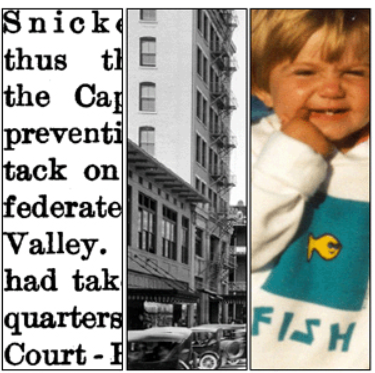
\includegraphics[width=0.7\linewidth]{Images/Week 3/bitdepth.png}
    \caption{Left to right - 1-bit bitonal, 8-bit grayscale, and 24-bit color images.}
\end{figure}
There is a square relationship between bit depth and file size, since doubling the depth results in twice the number of pixels in the x- and y-direction, so increasing the quality of the image drastically increases the size of the file and potentially complexity of transmitting the image.
\newline \newline
Additionally, \textbf{dynamic range} is the range of tonal difference between the lightest light and darkest dark of an image. The higher the dynamic range, the more potential shades can be represented, although the dynamic range does not automatically correlate to the number of tones reproduced.
\newline \newline
Finding a good balance between quality and file size will be very important during testing. Fortunately, lossless file formats like JPEG can reduce the size by ~10\% with an acceptable loss in image quality. 

% -----------------------
% WEEK 4
% -----------------------

\section{Embedded Control, Streaming and Interfaces}

\subsection{Communication Protocols}
\subsubsection{I2C}
For understanding the I2C protocol, \href{https://www.youtube.com/watch?v=CAvawEcxoPU&t=419s}{this video} is an excellent introduction.
Alternatively, \href{https://www.ti.com/lit/an/slva704/slva704.pdf?ts=1752540634031&ref_url=https%253A%252F%252Fwww.google.com%252F}{this resource} from Texas Instruments for a text version.
\newline \newline
Register configuration is the process of controlling and customising the behaviour of a camera sensor by writing specific values to its internal memory-mapped registers using a communication protocol, usually I²C.
Within camera engineering, this configuration defines essential operational parameters of the sensor such as exposure time, gain, binning mode, standby state, frame timing and more.
These registers are not software-level settings but actual control points embedded in the sensor's hardware. Each image sensor comes with a register map, which lists register addresses, default values, bit fields and the function of each setting. Some of these documents are publicly available, while others may require a non-disclosure agreement.
\newline \newline
The device controlling the camera, such as a microcontroller, system-on-chip or FPGA, acts as the I²C master and communicates with the sensor, which functions as the I²C slave. 
The master begins communication by sending a START condition on the I²C bus, followed by the 7-bit sensor address and a write bit. It then sends the register address to be configured, which may be 8 or 16 bits depending on the sensor, followed by the value to be written.
The sensor acknowledges receipt of each byte, and the master completes the sequence with a STOP condition. For some configurations, it is also possible to read back registers. This involves sending a repeated START, followed by the read bit, which allows the host to verify values or check sensor status.
\newline \newline
A typical initialisation sequence begins by placing the sensor into standby mode, then configuring essential functions such as internal clocks or PLLs, exposure control, analogue gain, timing settings like line and frame length, and any special modes such as binning or test patterns.
Once these values are set, the sensor is brought out of standby and begins streaming image data. This sequence is usually implemented in firmware and triggered at power-up. It is important to match the voltage levels of the I²C bus with the sensor's logic levels, as many sensors operate at 1.8 volts, and to include suitable pull-up resistors on the data and clock lines.
Careful attention to the sensor's timing requirements and register map ensures reliable communication and correct operation. Register configuration is a foundational task in camera development, enabling all further control over image capture and performance.

\subsubsection{SPI}
\href{https://www.youtube.com/watch?v=0nVNwozXsIc}{This resource} is a fantastic way to learn more about the fundamentals of SPI.
\newline \newline
SPI, or Serial Peripheral Interface, is another common communication protocol used to configure image sensors, though it is less frequently used than I²C in most commercial camera modules. Like I²C, SPI allows a controlling device, such as a microcontroller, FPGA or system-on-chip, to communicate directly with a sensor by reading from and writing to its internal registers.
SPI operates using four main lines: SCLK (serial clock), MOSI (master out, slave in), MISO (master in, slave out), and a dedicated chip select line, often referred to as CS or SS.
Unlike I²C, which is half-duplex and shared over two wires with address-based selection, SPI is full-duplex and uses separate lines for each direction of data transfer, with each slave selected individually via its chip select line.
\newline \newline
In the context of register configuration, SPI provides a simple and fast method for transmitting data to the sensor. To write a register, the host device pulls the chip select line low, then sends a command byte that typically includes a write flag and the target register address, followed by the data to be written.
For a read operation, the host sends a command indicating a read request along with the desired register address, and the sensor responds with the requested value.
Each SPI transaction is completed by pulling the chip select line high again. The format of the command and data sequences is specific to each sensor and is defined in its datasheet or register map documentation.
\newline \newline
SPI offers higher bandwidth than I²C and supports faster data rates, making it suitable for applications where timing precision or high-speed configuration is required. It is also simpler to implement in hardware due to its lack of bus arbitration and open-drain signalling.
However, SPI lacks standardised addressing, meaning it typically only supports one-to-one or one-to-few connections, and it requires more signal lines than I²C.
In camera systems, SPI is more commonly found in specialised or high-speed sensors, or in cases where deterministic timing and low latency are needed. Just like with I²C, SPI-based register configuration is a critical part of sensor integration, allowing the host to initialise and control core imaging parameters through direct low-level communication.

\subsubsection{I2C vs. SPI}

\begin{itemize}
    \item \textbf{Wiring and routing}
    \begin{itemize}
        \item I\textsuperscript{2}C uses only two wires (SDA and SCL), which simplifies PCB layout and reduces pin usage.
        \item SPI requires four lines (MOSI, MISO, SCLK, CS) and additional chip select lines for multiple devices, increasing routing complexity.
    \end{itemize}

    \item \textbf{Device addressing}
    \begin{itemize}
        \item I\textsuperscript{2}C supports addressing multiple devices on a shared bus using 7-bit or 10-bit addresses.
        \item SPI does not have built-in addressing; each peripheral must be selected individually with a separate chip select line.
    \end{itemize}

    \item \textbf{Data rate and performance}
    \begin{itemize}
        \item I\textsuperscript{2}C typically supports up to 400kHz (standard mode) or 1MHz+ (fast mode), which is sufficient for configuration tasks.
        \item SPI supports much higher clock speeds (10MHz or more), enabling faster data transmission and lower latency.
    \end{itemize}

    \item \textbf{Robustness and reliability}
    \begin{itemize}
        \item I\textsuperscript{2}C is more sensitive to noise due to open-drain signalling and bus capacitance, which can be a concern in noisy or long-trace CubeSat environments.
        \item SPI uses push-pull signalling and dedicated lines, which can offer better noise immunity and timing reliability.
    \end{itemize}

    \item \textbf{Scalability in small systems}
    \begin{itemize}
        \item I\textsuperscript{2}C scales well for multiple low-speed peripherals, making it ideal when multiple devices share a bus.
        \item SPI becomes less scalable with multiple devices due to chip select requirements and pin limitations in compact CubeSat PCBs.
    \end{itemize}
\end{itemize}

\subsection{Sensor Initialisation and Register Configuration}
We will use the Sony IMX sensor discussed in \ref{sec:sony-imx}.
\newline \newline
This sensor uses the \textbf{Camera Control Interface (CCI) protocol}, a subset of the I2C protocol, specifically designer for controlling caera modules in embedded systems. It allows a \href{https://en.wikipedia.org/wiki/Baseband_processor}{baseband processor} to communicate wit and control the camera's functions, such as image capture, resolution and other settings.
It is a two-wire, half-duplex, serial interface that supports 7-bit slave addressing and can handle multiple slaves at once on the same bus. It is also compatible with the I2C fast mode (400kHz).
Typically, the camera module acts as a slave device on the CCI bus, while the baseband processor acts as the master.
\newline \newline
You can initialise the sensor using the Tegra X1 Jetson Linux Driver using the guide found \href{https://developer.ridgerun.com/wiki/index.php/Sony_IMX219_Linux_driver}{here}.
\newline
To convert the naked Bayer grid data into RGB data, we can use Bayer2rgb. There are a few choices of interpolation, however, they differ very little. It can output .tiff files and can integrate with ImageMagick to output other formats.
\verb|gst-launch-1.0 -v v4l2src device=/dev/video0 num-buffers=1 ! "video/x-bayer, format=rggb, width=3280, height=2464" ! filesink location=test_3280x2464.bayer |
\verb|./bayer2rgb --input=test_3280x2464.bayer --output=data.tiff --width=3296 --height=2464 --bpp=16 --first=RGGB --method=BILINEAR --tiff |
And to convert from .tiff to another file format, like .png:
\begin{verbatim}
convert data.tiff data.png
\end{verbatim}
The above process captures images in 3280x2464 resolution, however, this resolution can be changed by adjusting the \verb|width| and \verb|height| parameters.




































































\end{multicols}

\end{document}